%   Filename    : chapter_4.tex 
\chapter{Results and Discussion}
\section{Data Gathering}
The data for dengue case prediction was gathered from a variety of reliable sources, enabling a comprehensive dataset spanning from January 2011 to October 2024. This dataset includes 720 rows of data, each containing weekly records of dengue cases along with corresponding meteorological variables, such as rainfall, temperature, and humidity.
\begin{enumerate}
	\item Dengue Case Data: The primary source of historical dengue cases came from the Humanitarian Data Exchange and the Western Visayas Center for Health Development (WVCHD). The dataset, accessed through Freedom of Information (FOI) requests, provided robust case numbers for the Western Visayas region. The systematic collection of these data points was essential for establishing a reliable baseline for model training and evaluation.
	\item Weather Data: Weekly weather data was obtained by web scraping from Weather Underground, allowing access to rainfall, temperature, wind, and humidity levels that correlate with dengue prevalence.
\end{enumerate}
\begin{table}[h!]
	\centering
	\resizebox{1\textwidth}{!}{%
		\begin{tabular}{|l|c|c|c|c|c|c|c|}
			\hline
			\textbf{Time} & \textbf{Rainfall} & \textbf{MaxTemperature} & \textbf{AverageTemperature} & \textbf{MinTemperature} & \textbf{Wind} & \textbf{Humidity} & \textbf{Cases} \\ 
			\hline
			2011-01-03 & 9.938571 & 29.444400 & 25.888890 & 23.888900 & 11.39 & 86.242857 & 5 \\ 
			\hline
			2011-01-10 & 8.587143 & 30.000000 & 26.705556 & 24.444444 & 7.32 & 88.028571 & 4 \\ 
			\hline
			2011-01-17 & 5.338571 & 30.000000 & 26.616667 & 25.000000 & 7.55 & 84.028571 & 2 \\ 
			\hline
			2011-01-24 & 5.410000 & 30.555556 & 26.483333 & 20.555556 & 10.67 & 80.971429 & 7 \\ 
			\hline
			2011-01-31 & 2.914286 & 28.333333 & 25.283333 & 18.650000 & 11.01 & 74.885714 & 2 \\ 
			\hline
		\end{tabular}%
	}
	\caption{Snippet of the combined dataset}
	\label{tab:data_snippet}
\end{table}
\section{Exploratory Data Analysis}

From Table \ref{tab:data_schema}, the dataset consists of 720 weekly records with 8 columns:
\begin{itemize}
	\item \textbf{Time.} Weekly timestamps (e.g. ``2011-w1'')
	\item \textbf{Rainfall.} Weekly average rainfall (mm)
	\item \textbf{MaxTemperature, AverageTemperature, MinTemperature.} Weekly temperature data (°C)
	\item \textbf{Wind.} Wind speed (m/s)
	\item \textbf{Humidity.} Weekly average humidity (\%)
	\item \textbf{Cases.} Reported dengue cases
\end{itemize}

\begin{table}[h!]
	\centering
	\begin{tabular}{|c|l|c|c|}
		\hline
		\textbf{\#} & \textbf{Column} & \textbf{Non-Null Count} & \textbf{Data Type} \\
		\hline
		0 & Time & 720 non-null & datetime64[ns] \\
		\hline
		1 & Rainfall & 720 non-null & float64 \\
		\hline
		2 & MaxTemperature & 720 non-null & float64 \\
		\hline
		3 & AverageTemperature & 720 non-null & float64 \\
		\hline
		4 & MinTemperature & 720 non-null & float64 \\
		\hline
		5 & Wind & 720 non-null & float64 \\
		\hline
		6 & Humidity & 720 non-null & float64 \\
		\hline
		7 & Cases & 720 non-null & int64 \\
		\hline
	\end{tabular}
	\caption{Data Schema: Column Names, Non-Null Counts, and Data Types}
	\label{tab:data_schema}
\end{table}


From the statistics in Table \ref{tab:summary_statistics}, the number of cases ranges from 0 to 319. The average number of dengue cases per week is 23.74, with a median of 12 cases and a standard deviation of 37.14. The distribution is highly skewed, with some weeks experiencing significant number of cases (up to 319 cases). Rainfall shows a wide variation (0 to 445mm), while temperature remains relatively stable, with an average of 28.1 degree celsius. Humidity levels ranges from 73\% to 89\% with a mean of 81.6\%.

\begin{table}[h!]
	\centering
	\resizebox{1\textwidth}{!}{%
		\begin{tabular}{|l|c|c|c|c|c|c|c|c|}
			\hline
			\textbf{Statistic} & \textbf{Time} & \textbf{Rainfall} & \textbf{MaxTemperature} & \textbf{AverageTemperature} & \textbf{MinTemperature} & \textbf{Wind} & \textbf{Humidity} & \textbf{Cases} \\
			\hline
			\textbf{Count} & 720 & 720.000000 & 720.000000 & 720.000000 & 720.000000 & 720.000000 & 720.000000 & 720.000000 \\
			\hline
			\textbf{Mean} & 2017-12-02 11:22:00 & 13.957499 & 32.191142 & 28.110319 & 25.038472 & 6.172417 & 81.609442 & 23.744444 \\
			\hline
			\textbf{Min} & 2011-01-03 00:00:00 & 0.000000 & -14.600000 & 24.494444 & 12.222222 & 1.910000 & 73.185714 & 0.000000 \\
			\hline
			\textbf{25\%} & 2014-06-21 06:00:00 & 1.270000 & 31.666667 & 27.504167 & 25.000000 & 4.117500 & 79.885713 & 5.000000 \\
			\hline
			\textbf{50\% (Median)} & 2017-12-07 12:00:00 & 4.318000 & 32.222222 & 28.161111 & 25.000000 & 5.725000 & 81.771429 & 12.000000 \\
			\hline
			\textbf{75\%} & 2021-05-11 18:00:00 & 10.414000 & 32.777778 & 28.751389 & 25.555556 & 7.860000 & 83.503571 & 26.000000 \\
			\hline
			\textbf{Max} & 2024-10-28 00:00:00 & 445.008000 & 58.333333 & 30.916667 & 32.222222 & 19.200000 & 89.571429 & 319.000000 \\
			\hline
			\textbf{Std Dev} & N/A & 35.448846 & 2.616379 & 0.999800 & 1.291659 & 2.446703 & 2.831674 & 37.144813 \\
			\hline
		\end{tabular}%
	}
	\caption{Descriptive Statistics of the Combined Dataset}
	\label{tab:summary_statistics}
\end{table}


Figure \ref{fig:data_trend} illustrates the trend of weekly dengue cases over time. The data reveals periodic spikes in the number of cases, suggesting a seasonal pattern in dengue cases. Notably, peak cases are observed during certain periods approximately 3 years, potentially aligning with specific climatic conditions such as increased rainfall or temperature changes. This underscores the importance of incorporating climate variables into the forecasting model.

\begin{figure}[ht]
	\centering
	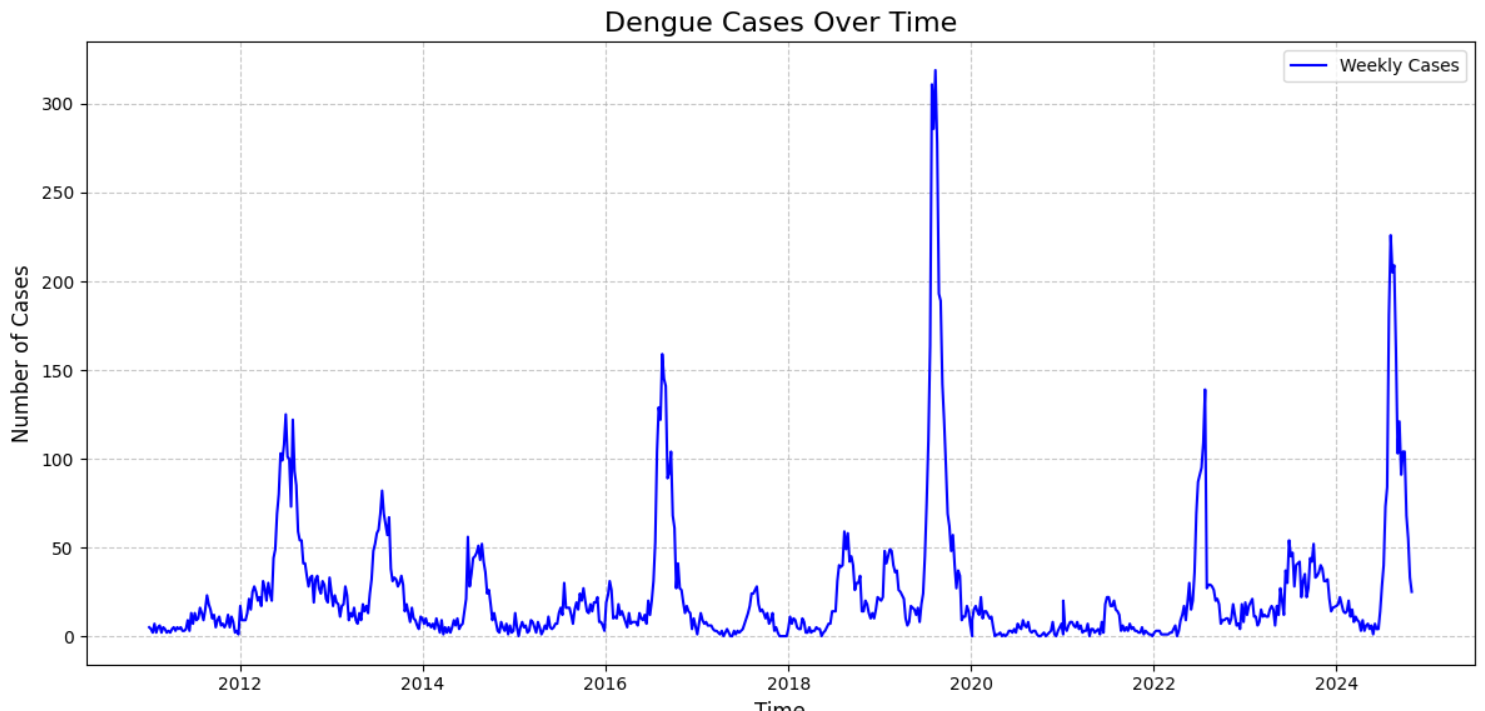
\includegraphics[width=0.90\textwidth]{dengue_trend}
	\caption{Trend of Dengue Cases}
	\label{fig:data_trend}
\end{figure}

Figure \ref{fig:rainfallVScases} presents a time series subplot that combines rainfall and dengue cases to highlight potential non-linear associations between the two variables. In this figure, raw rainfall data is represented by blue scatter points (aligned with the left y-axis), while a blue solid line traces its 4-week rolling average to reveal underlying trends. Simultaneously, the red dashed line illustrates the smoothed trajectory of dengue cases (aligned with the right y-axis), also using a 4-week rolling average to reduce short-term fluctuations and emphasize longer-term patterns.

Notably, the plot suggests a recurring pattern. Periods of increased rainfall often precede or coincide with spikes in dengue cases. This observed relationship supports existing literature which proposes that higher rainfall contributes to the proliferation of mosquito breeding sites, particularly in stagnant water, thereby elevating the risk of dengue transmission.

\begin{figure}[ht]
	\centering
	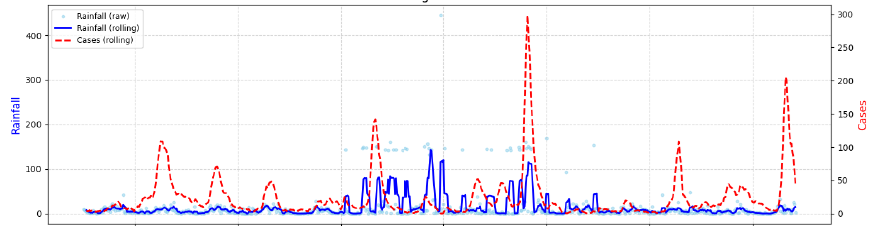
\includegraphics[width=0.7\textwidth]{rainfallVScases}
	\caption{Rainfall and Dengue Cases Over Time}
	\label{fig:rainfallVScases}
\end{figure}

The KDE plots in Figure \ref{fig:KDE} illustrate the distributions of meteorological variables during outbreak and normal dengue weeks. The x-axes represent the actual values of each feature, while the y-axes show density, indicating how frequently values occur within each category. The graphs reveal that outbreak weeks tend to have moderately higher rainfall than weeks with no outbreak. This is evident in the way the curve for outbreak weeks is positioned slightly to the right of the curve for normal weeks. In terms of temperature, the distributions for both normal and outbreak weeks appear very similar; however, upon closer inspection, the curve for maximum temperature shows a slightly higher density at higher values during outbreak weeks. The same is true for humidity, with outbreak weeks showing greater density at higher humidity levels. These patterns suggest that dengue outbreaks are more likely to occur during warm, humid periods with relatively high rainfall. Based on these observations, rainfall, maximum temperature, and humidity were selected as the meteorological features for training the predictive models.


\begin{figure}[ht]
	\centering
	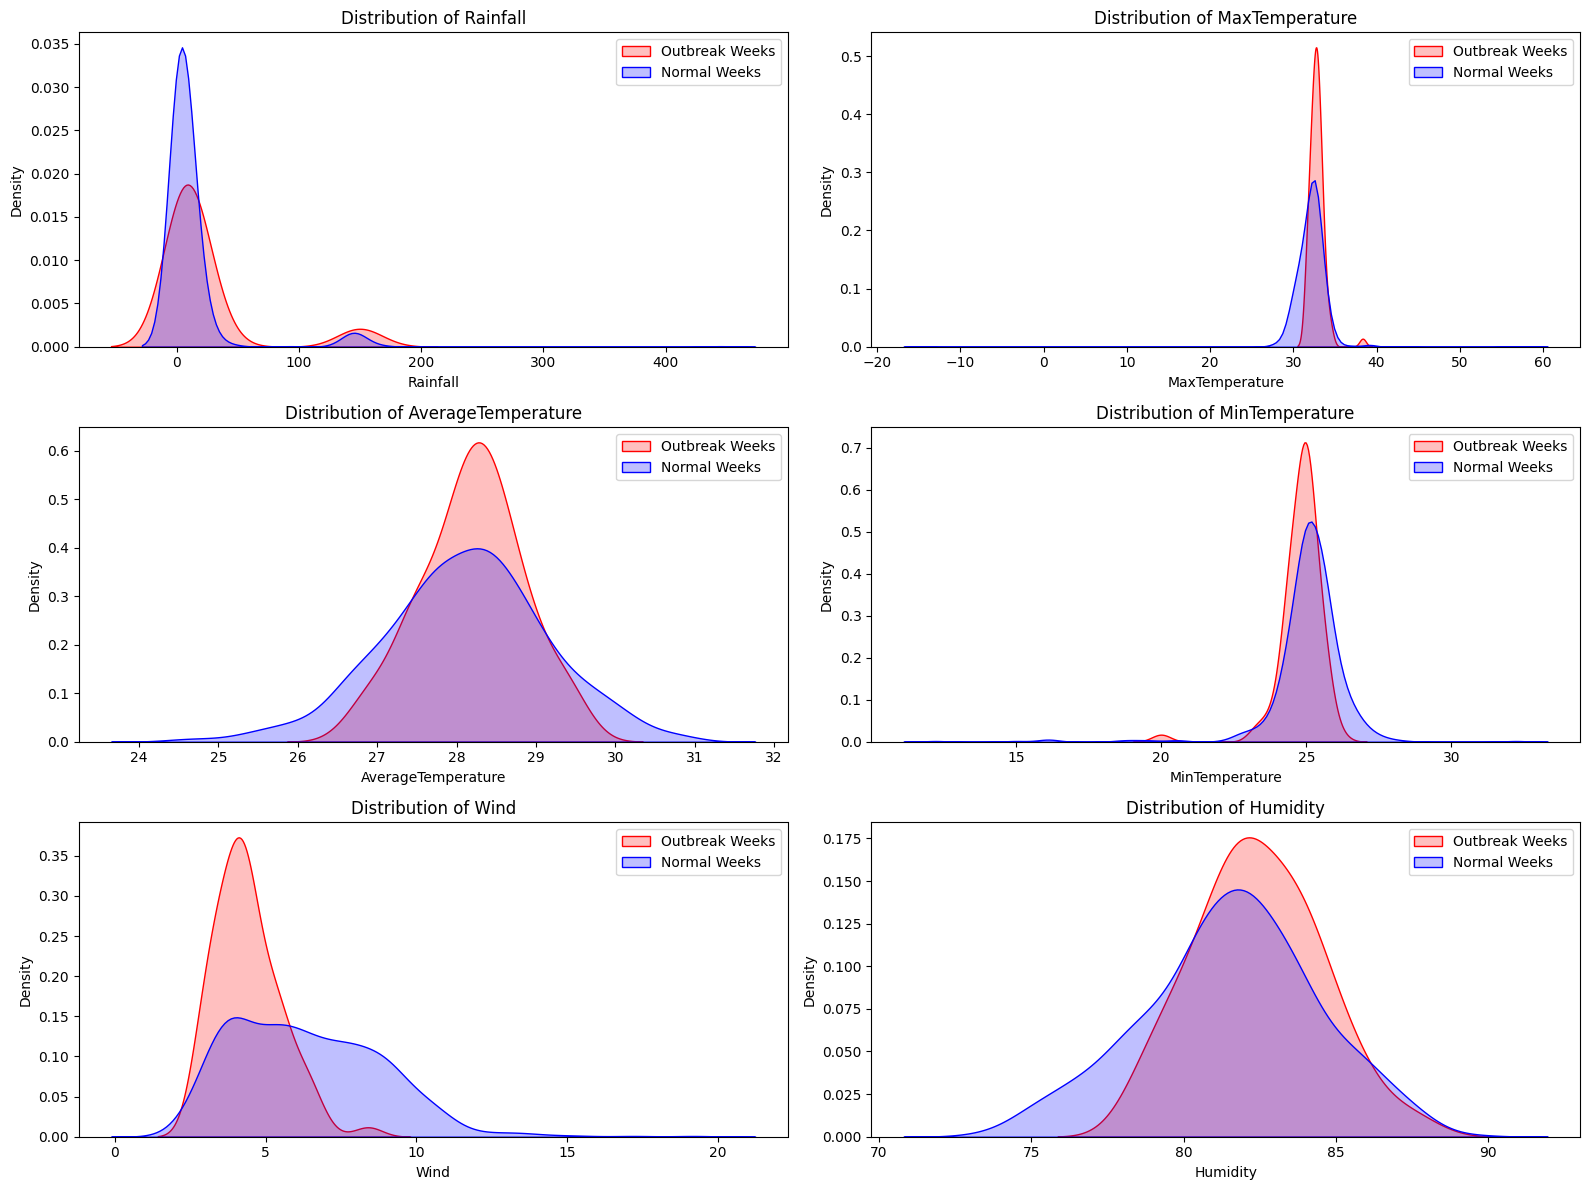
\includegraphics[width=1\textwidth]{KDE}
	\caption{Kernel Density Estimate Plots of Meteorological Features}
	\label{fig:KDE}
\end{figure}

\clearpage

\section{Outbreak Detection}
To identify outbreaks, the researchers calculated the outbreak threshold value using the historical mean as the endemic channel. The threshold is determined using the formula:  

\begin{align}  
	\text{Outbreak Threshold Value} &= \mu + 2\sigma \\  
	&= 23.744444 + 2(37.144813) \\  
	&= 23.744444 + 74.289626 \\  
	&= 98.03407  
\end{align}  

where \(\mu\) is the historical mean and \(\sigma \) is the standard deviation.

This result indicates that dengue cases exceeding 98 in Iloilo City can be considered an outbreak. However, it is important to note that this threshold serves only as a baseline. 

\section{Model Training Results}

The models were evaluated using three commonly used regression metrics: Mean Squared Error (MSE), Root Mean Squared Error (RMSE), and Mean Absolute Error (MAE). These metrics help assess how accurately each model forecasts dengue cases based on historical data. Table \ref{tab:comparison_of_models} presents a comparative analysis of the models using these metrics.
\begin{itemize}
	\item \textbf{MSE} represents the average of the squared differences between predicted and actual values. It penalizes larger errors more heavily.
	\item \textbf{RMSE}, the square root of MSE, provides a more interpretable value in the same units as the target (i.e., number of dengue cases).
	\item \textbf{MAE} calculates the average magnitude of the errors without considering their direction, giving a more straightforward understanding of the average prediction error.
\end{itemize}

In simpler terms, lower values in these metrics indicate that the model is making more accurate predictions.

\begin{table}[h!]
	\centering
	\resizebox{1\textwidth}{!}{%
		\begin{tabular}{|l|c|c|c|c|c|}
			\hline
			\textbf{Method} & \textbf{LSTM} & \textbf{Seasonal ARIMA} & \textbf{ARIMA} & \textbf{Kalman Filter} & \textbf{KF-LSTM} \\ 
			\hline
			\textbf{Testing MSE}   & 406.03 & 1261.20 & 1521.48 & 1474.82 & 785.35 \\ 
			\hline
			\textbf{Testing RMSE}  & 20.15  & 34.45  & 39.00 & 38.40 & 25.56 \\ 
			\hline
			\textbf{Testing MAE}   & 12.61  & 18.73  & 25.80 & 22.33 & 14.55 \\ 
			\hline
			\textbf{Best Parameters}   
			& \begin{tabular}[c]{@{}c@{}}Window Size: 5\\ Learning Rate: 0.01\\ Units: 64\end{tabular}  
			& (2,0,2)(0,1,1)  
			& (1,2,2) 
			& \begin{tabular}[c]{@{}c@{}}Observation Covariance: 10.0\\ Transition Covariance: 0.1 $\times$ Identity\end{tabular}
			& Same as LSTM \\ 
			\hline
		\end{tabular}%
	}
	\caption{Comparison of different models for dengue prediction}
	\label{tab:comparison_of_models}
\end{table}

As shown in Table \ref{tab:comparison_of_models}, the LSTM model consistently achieved the lowest MSE (406.03), RMSE (20.15), and MAE (12.61) among all evaluated models. This suggests that, on average, the LSTM’s predictions were about 12 to 20 cases away from the actual values, which is a strong indication of reliability for practical use in public health decision-making.

In contrast, traditional time series models like Seasonal ARIMA and ARIMA showed higher errors, indicating less accurate predictions. For example, the Seasonal ARIMA model had an RMSE of 34.45, which implies that its forecasts deviated from actual dengue case counts by around 34 cases on average, a significant discrepancy for health officials planning resource allocation.

The Kalman Filter and hybrid KF-LSTM models showed moderate performance. Although they did not outperform LSTM, the hybrid model (KF-LSTM) still reduced errors compared to the standalone Kalman Filter.

These results highlight the potential of LSTM-based models to provide timely and accurate forecasts that can support early intervention, resource planning, and policy formulation to combat dengue outbreaks in Iloilo City.

\subsection{LSTM Model}
The LSTM model was tuned for the following parameters: learning rate and units. The hyperparameter tuning was conducted for each window size, finding the best parameters for each window size. Further evaluating which window size is most suitable for the prediction model, Table \ref{tab:comparison_of_lstm} shows the evaluation metrics for each window size used in the LSTM model training.
\begin{table}[h!]
	\centering
	\begin{tabular}{|l|c|c|c|c|}
		\hline
		\textbf{Window Size} & \textbf{MSE} & \textbf{RMSE} & \textbf{MAE} & \textbf{R²}\\ \hline
		\textbf{5} & \textbf{406.03} & \textbf{20.15} & \textbf{12.61} & \textbf{0.76}\\ \hline
		\textbf{10} & \textbf{1037.77} & \textbf{32.21} & \textbf{26.79} & \textbf{0.39}\\ \hline
		\textbf{20} & \textbf{427.39} & \textbf{20.67} & \textbf{13.61} & \textbf{0.75}\\ \hline
	\end{tabular}
	\caption{Comparison of Window Sizes}
	\label{tab:comparison_of_lstm}
\end{table}

The results indicate that a window size of 5 weeks provides the most accurate predictions, as evidenced by the lowest MSE and RMSE values. Furthermore, the R² score of 0.76 indicates that 76\% of the variability in the target variable (cases) is explained by the independent variables (the inputs) in the model, making it a reliable configuration overall.

As shown in Table \ref{tab:tcsv_lstm_table}, the results from time series cross-validation indicate consistent performance trends, with a window size of 5 yielding the highest average RMSE across all folds compared to the other window sizes.

\begin{table}[h!]
	\centering
	\begin{tabular}{|l|c|c|c|}
		\hline
		\textbf{Window Size} & \textbf{Average RMSE} & \textbf{Average MAE} & \textbf{Average R²}\\ \hline
		\textbf{5} & \textbf{16.69} & \textbf{9.06} & \textbf{0.79}\\ \hline
		\textbf{10} & \textbf{17.08} & \textbf{10.40} & \textbf{0.75}\\ \hline
		\textbf{20}& \textbf{16.93} & \textbf{8.75} & \textbf{0.81}\\ \hline
	\end{tabular}
	\caption{Time-Series Cross Validation Results: Comparison of Window Sizes}
	\label{tab:tcsv_lstm_table}
\end{table}

Figure \ref{fig:tcsv_training} illustrates the model’s performance in predicting dengue cases for each fold using a window size of 5. As shown in the plot, the training set progressively increases with each fold, mimicking a real-world scenario where more data becomes available over time for dengue prediction. Figure \ref{fig:tcsv_testing} demonstrates that the predicted cases closely follow the trend of the actual cases, indicating that the LSTM model successfully captures the underlying patterns in the data. It is also evident that as the fold number increases and the training set grows, the accuracy of the predictions on the test set improves. Despite the test data being unseen, the model exhibits a strong ability to generalize, suggesting it effectively leverages past observations to predict future trends.

\begin{figure}[H]
	\centering
	\includegraphics[width=1\textwidth]{TSCV_training}
	\caption{Training Folds - Window Size 5}
	\label{fig:tcsv_training}
\end{figure}

\begin{figure}[H]
	\centering
	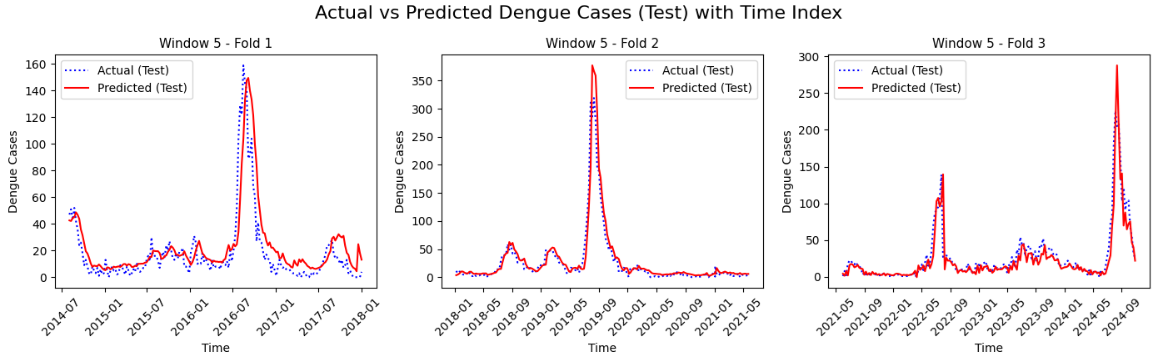
\includegraphics[width=1\textwidth]{TCSV_testing}
	\caption{Testing Folds - Window Size 5}
	\label{fig:tcsv_testing}
\end{figure}

\subsection{ARIMA Model}

The ARIMA model was developed to capture non-seasonal trends in the data. To determine the best model configuration, grid search was used to explore various combinations of ARIMA parameters, ultimately selecting \textbf{ARIMA(1, 2, 2)}. The model was iteratively refined over \textbf{400 iterations} to ensure convergence to an optimal solution. Figure \ref{fig:Arima_result} illustrates the comparison between actual and predicted dengue cases in the test set. As shown in the plot, the ARIMA model struggled to capture the non-linear characteristics and abrupt spikes in the data. Consequently, it failed to accurately reflect the fluctuations and outbreak patterns seen in the actual case counts.

\begin{figure}[H]
	\centering
	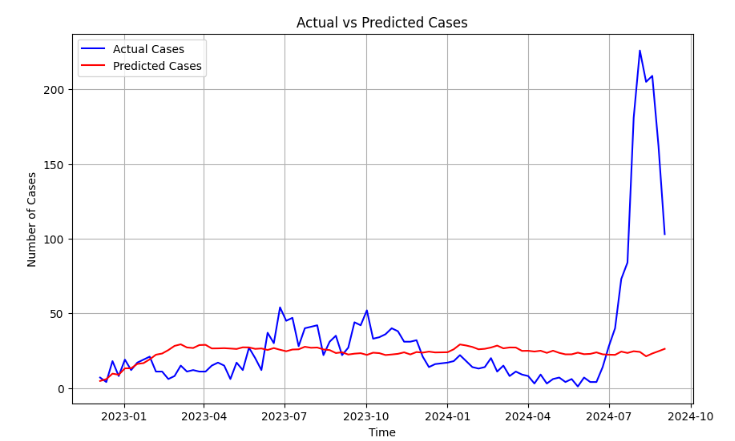
\includegraphics[width=1\textwidth]{line_graph_Arima}
	\caption{ARIMA Prediction Results for Test Set}
	\label{fig:Arima_result}
\end{figure}

The model's performance was assessed using regression metrics to evaluate its forecasting capability. The ARIMA model yielded the following error metrics:

\begin{itemize}
	\item \textbf{MSE (Mean Squared Error)}: 1521.48
	\item \textbf{RMSE (Root Mean Squared Error)}: 39.01
	\item \textbf{MAE (Mean Absolute Error)}: 25.80
\end{itemize}

\subsection{Seasonal ARIMA (SARIMA) Model}

To address the limitations of the ARIMA model, a Seasonal ARIMA (SARIMA) model was developed to capture both non-seasonal and seasonal variations in the data.

This model incorporates seasonal parameters, which were tuned using grid search to find the best configuration: \textbf{SARIMA(2, 0, 2)(0, 1, 1)[52]}. As with ARIMA, \textbf{400 iterations} were applied to ensure a robust fit. As shown in Figure \ref{fig:Sarima_result}, the SARIMA model demonstrates a notable improvement in performance. Unlike its non-seasonal counterpart, it effectively captures the general trend and aligns more closely with the peaks observed in the actual dengue cases, indicating its ability to model seasonal dynamics.

\begin{figure}[H]
	\centering
	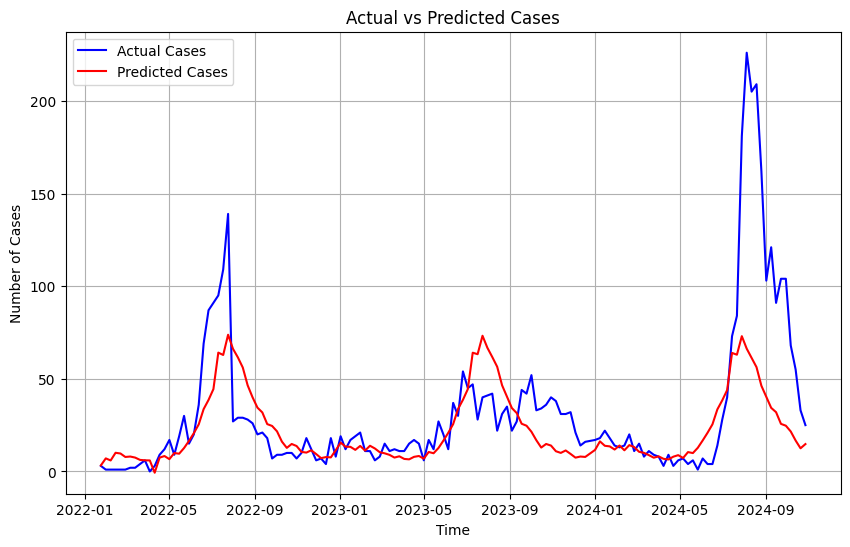
\includegraphics[width=1\textwidth]{line_graph_Sarima}
	\caption{Seasonal ARIMA Prediction Results for Test Set}
	\label{fig:Sarima_result}
\end{figure}

The model's performance was assessed using regression metrics to evaluate its forecasting capability. The SARIMA model yielded the following error metrics: \begin{itemize} \item \textbf{MSE}: 1109.69 \item \textbf{RMSE}: 33.31 \item \textbf{MAE}: 18.09 \end{itemize} The lower error values, when compared to the ARIMA model, highlight the SARIMA model's superior capability in forecasting dengue cases. Its effectiveness in capturing seasonal patterns contributed to a more accurate representation of the actual cases.

After training the model, the SARIMA model was validated using the same Time Series Cross-Validation strategy employed in the LSTM model. Table \ref{tab:tcsv_sarima} presents the performance metrics for each fold, as well as the average metrics across all folds. The average RMSE and MAE values were close to those obtained during the initial training phase, indicating that the SARIMA model performed consistently across different time segments.

\begin{table}[h!]
	\centering
	\begin{tabular}{|l|c|c|c|}
		\hline
		\textbf{Fold} & \textbf{MSE} & \textbf{RMSE} & \textbf{MAE} \\
		\hline
		1 & 659.68  & 25.68 & 16.00 \\
		2 & 2127.49 & 46.12 & 21.30 \\
		3 & 996.43  & 31.56 & 18.89 \\
		\hline
		\textbf{Average} & \textbf{1261.20} & \textbf{34.45} & \textbf{18.73} \\
		\hline
	\end{tabular}
	\caption{Comparison of SARIMA performance for each fold}
	\label{tab:tcsv_sarima}
\end{table}


\subsection{Kalman Filter Model}

Figure \ref{fig:Kalman_result} shows the comparison between the actual dengue cases and the predicted values on the test set. As illustrated in the plot, the Kalman Filter model demonstrates a moderate ability to follow the general trend of the actual data. While it effectively captures some rising and falling patterns, it still struggles to accurately replicate the sharp peaks and extreme values found in the real case counts. This limitation is particularly noticeable during the large spikes in 2022 and 2024. The model’s performance was evaluated using standard regression metrics. The results are as follows:
\[
\text{MSE} = 1474.82, \quad
\text{RMSE} = 38.40, \quad
\text{MAE} = 22.34
\]
\begin{figure}[H]
	\centering
	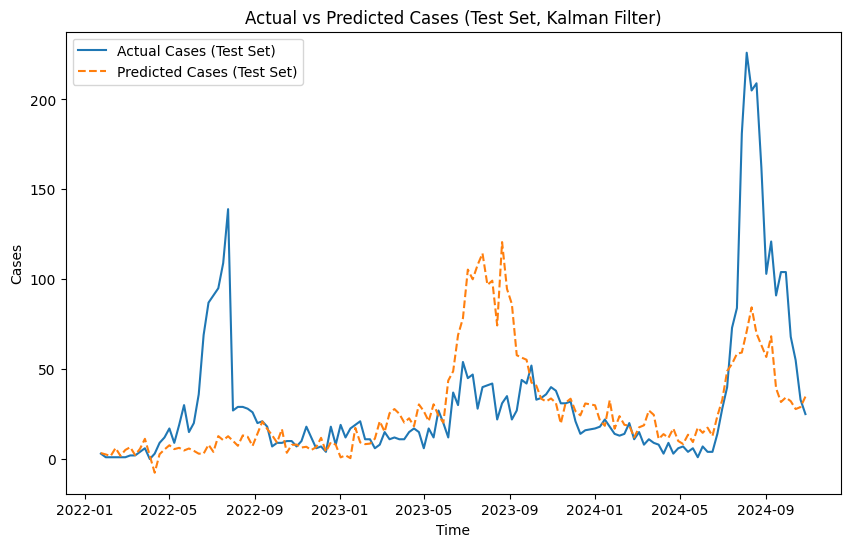
\includegraphics[width=1\textwidth]{line_graph_Kalman}
	\caption{Kalman Filter Prediction Results for Test Set}
	\label{fig:Kalman_result}
\end{figure}

The Kalman Filter was then combined with the LSTM model in order to see improvements in its predictions. Table \ref{tab:tcsv_kflstm} shows the metrics across three folds using the same Time Series Cross Validation Strategy employed in the previous models to see how it performed on different time segments.

\begin{table}[h!]
	\centering
	\begin{tabular}{|l|c|c|c|}
		\hline
		\textbf{Fold} & \textbf{MSE} & \textbf{RMSE} & \textbf{MAE} \\
		\hline
		1 & 113.59  & 10.66 & 6.42 \\
		2 & 752.51 & 27.43 & 12.11 \\
		3 & 1489.95  & 38.60 & 25.13 \\
		\hline
		\textbf{Average} & \textbf{785.35} & \textbf{25.56} & \textbf{14.55} \\
		\hline
	\end{tabular}
	\caption{Comparison of KF-LSTM performance for each fold}
	\label{tab:tcsv_kflstm}
\end{table}

As can be seen in the table above, the performance of the hybrid model demonstrated improvements in all metrics as compared to just using the Kalman Filter alone.

\section{Model Simulation}
To evaluate the LSTM model's real-world forecasting ability, a simulation was conducted to predict dengue cases for the year 2025. The model was retrained exclusively, using the parameters found from the initial training, on data from 2011 to January 2025, using both dengue cases and weather variables. Importantly, the actual dengue case values for 2025 were never included during training. Instead, only the weather variables collected for 2025 were input into the model to generate predictions for that year. After prediction, the forecasted dengue cases for 2025 were compared against the true observed cases to assess the model’s accuracy. Figure \ref{fig:modeltesting} shows that the predicted values closely follow the trend, although it may overestimate the dengue cases in some weeks. 

\begin{figure}[H]
	\centering
	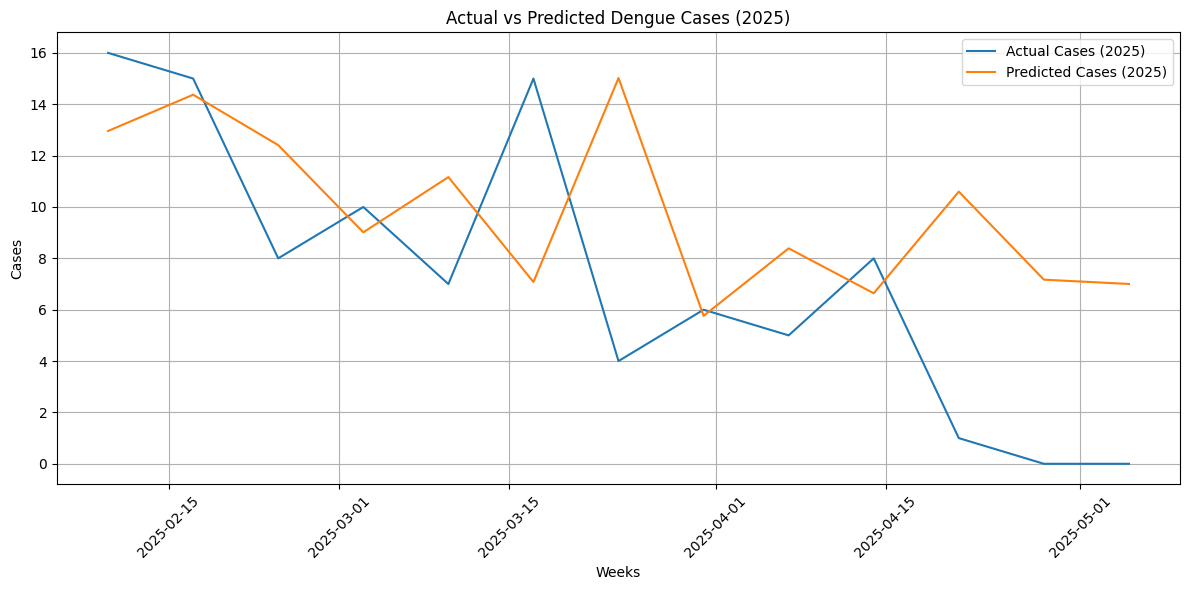
\includegraphics[width=1\textwidth]{modeltesting}
	\caption{Predicted vs Actual Dengue Cases 2025}
	\label{fig:modeltesting}
\end{figure}

Retraining the model is essential to ensure it remains accurate and responsive to the evolving trends of dengue case patterns over time. Ideally, the model should be updated whenever new data becomes available to capture recent dynamics. However, given the computational cost associated with retraining, a more practical approach is to update the model on a monthly basis. This allows the incorporation of approximately four weeks’ worth of new data, providing a meaningful update to the model’s predictive capabilities without excessive resource consumption. Furthermore, this schedule aligns with the typical data release cycle of provincial health offices, which, based on the researchers’ experience, usually occurs monthly. This balance between accuracy and efficiency ensures that the model remains both up-to-date and manageable in real-world deployment.

\section{System Prototype}
\subsection{Home Page}
The Home Page is intended for all visitors to the web application. The Analytics Dashboard, which displays relevant statistics for dengue cases at a certain time and location, is the primary component highlighted, as seen in Figure \ref{fig:home_page}. This component includes a combo chart that graphs the number of dengue cases and deaths per week in a specific year, a choropleth map that tracks the number of dengue cases per barangay in a location, and various bar charts that indicate the top constituent places affected by dengue. 

\begin{figure}[H]
	\centering
	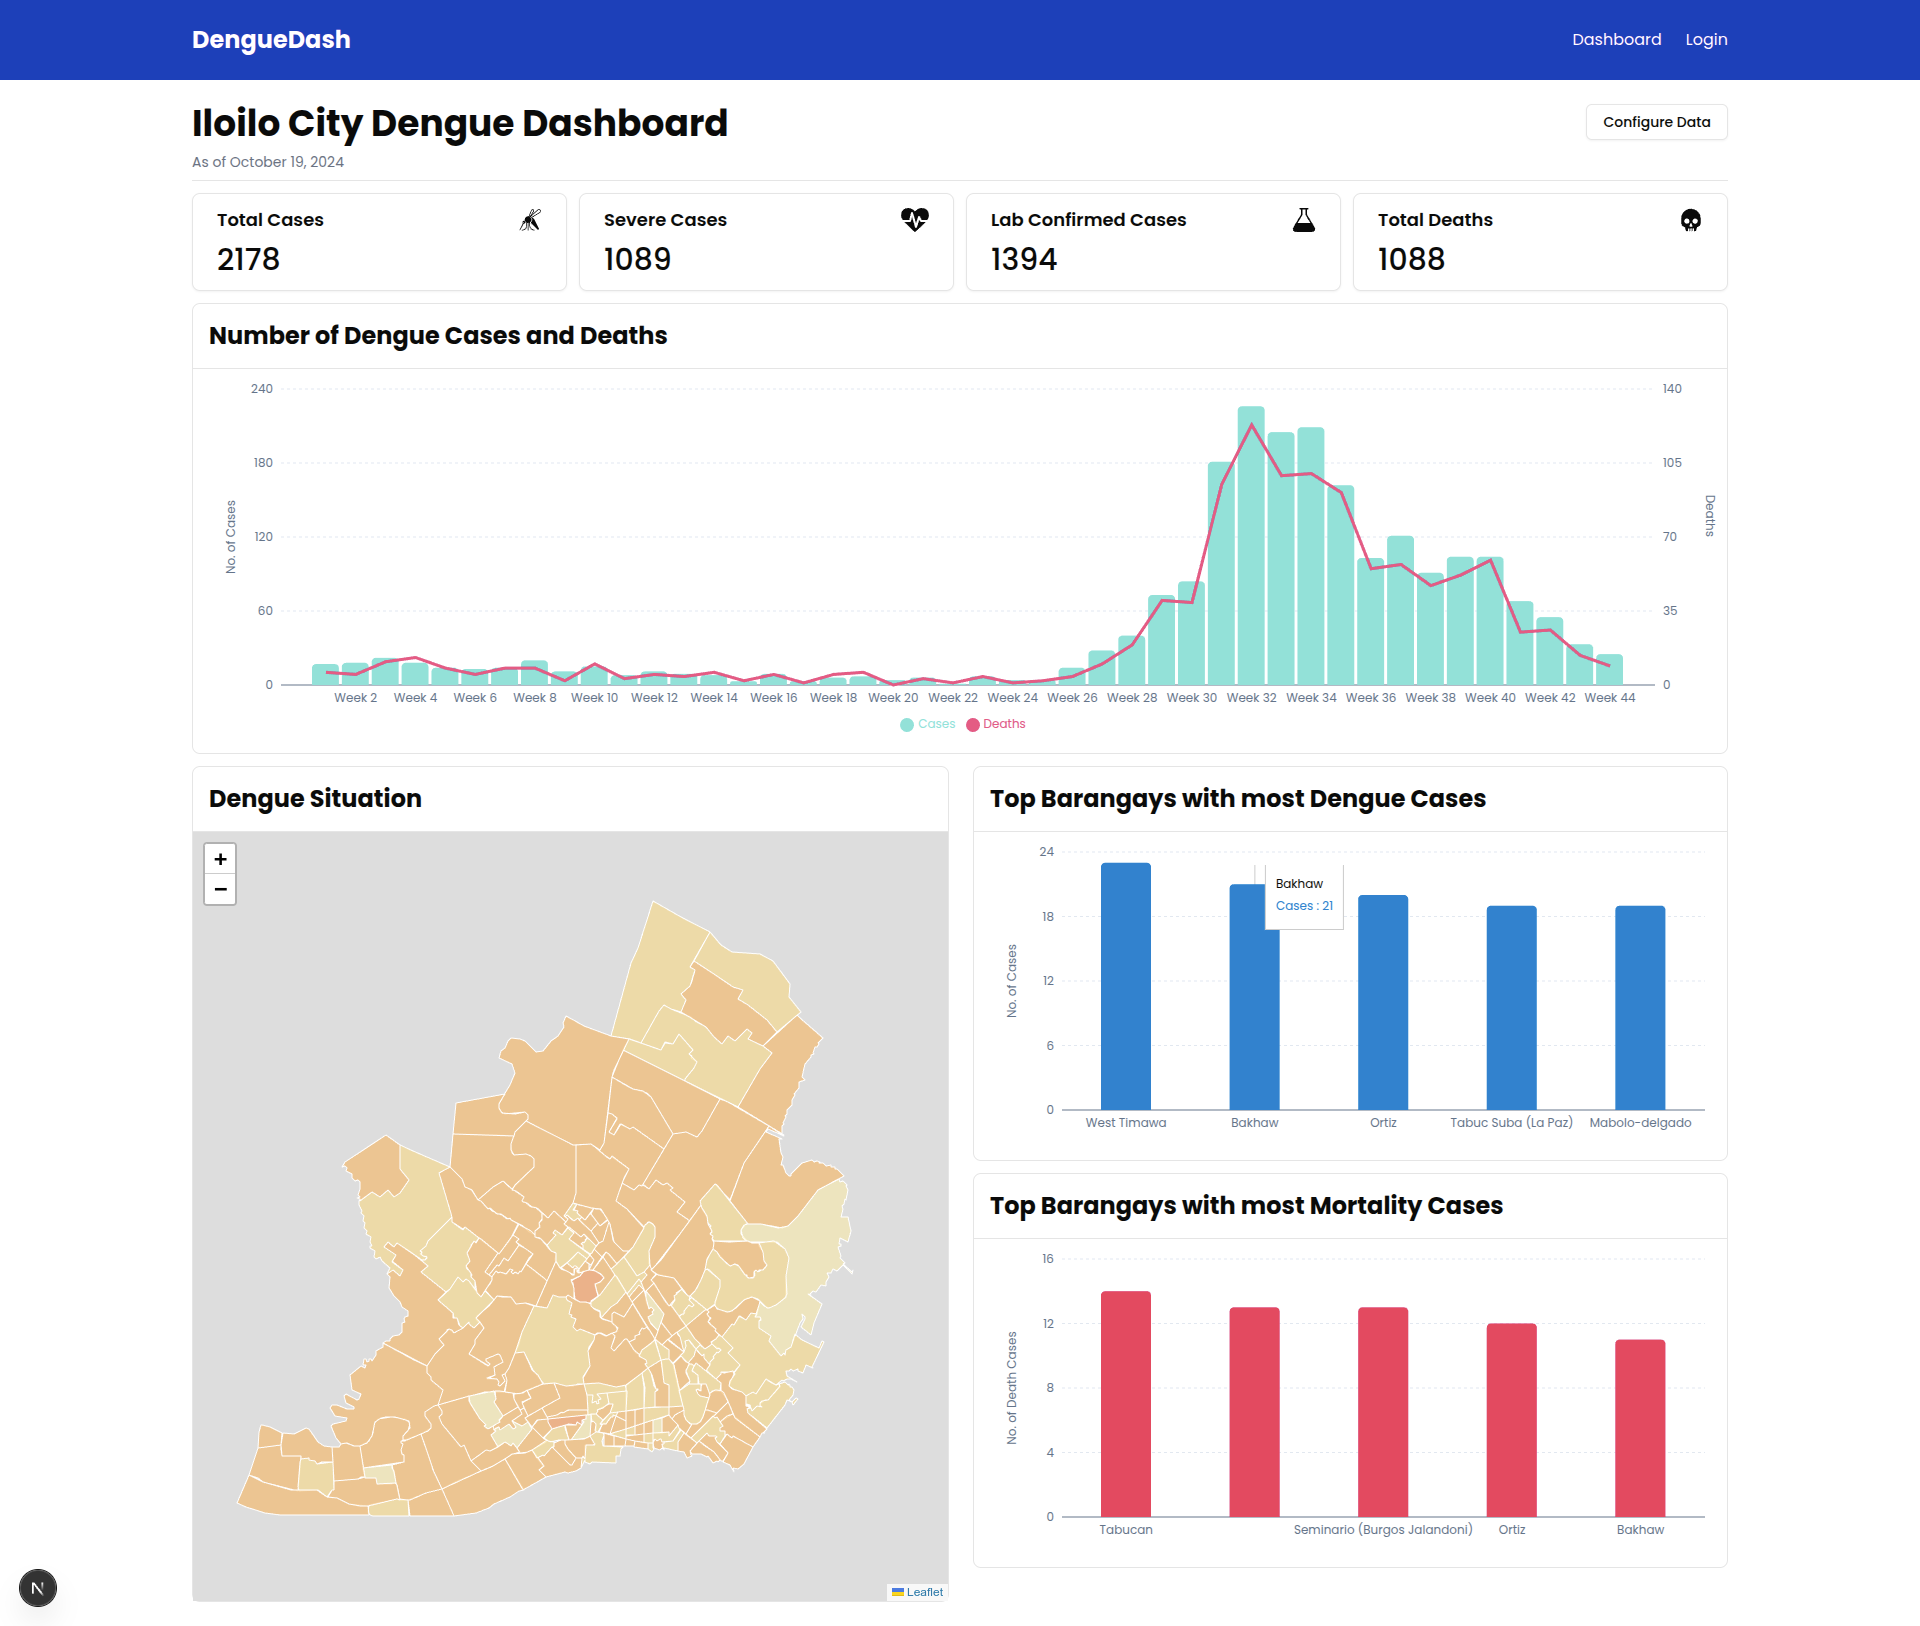
\includegraphics[width=0.8\textwidth, height=0.6\textheight, keepaspectratio]{home_page}
	\caption{Home Page}
	\label{fig:home_page}
\end{figure}

\subsection{User Registration, Login, and Authentication}
The registration page, as shown in \ref{fig:signup_page_1} and \ref{fig:signup_page_2}, serves as a gateway to access the authenticated pages of the web application. Only prospective encoders can register an account, as administrator accounts are created by existing administrator accounts to protect the integrity of the data in production. After registering, the "encoder account" cannot access the authorized pages yet as it needs to be verified first by an administrator managing the unit the user entered. Because of this, proper identification (user's picture and employee identification card) is mandatory to help the admins verify the identity of the registrant. Once verified, the user can log in to the system through the page shown in Figure \ref{fig:login_page}. After entering the correct credentials, which consist of an email and password, the system uses HTTP-only cookies containing JSON Web Tokens (JWT) to prevent vulnerability to Cross-site Scripting (XSS) attacks. It will then proceed to the appropriate page for the type of user it belongs to. Logging out, on the other hand, will remove both the access and refresh tokens from the browser and will blacklist the latter token to make it unusable for security purposes. 

\begin{figure}[H]
	\centering
	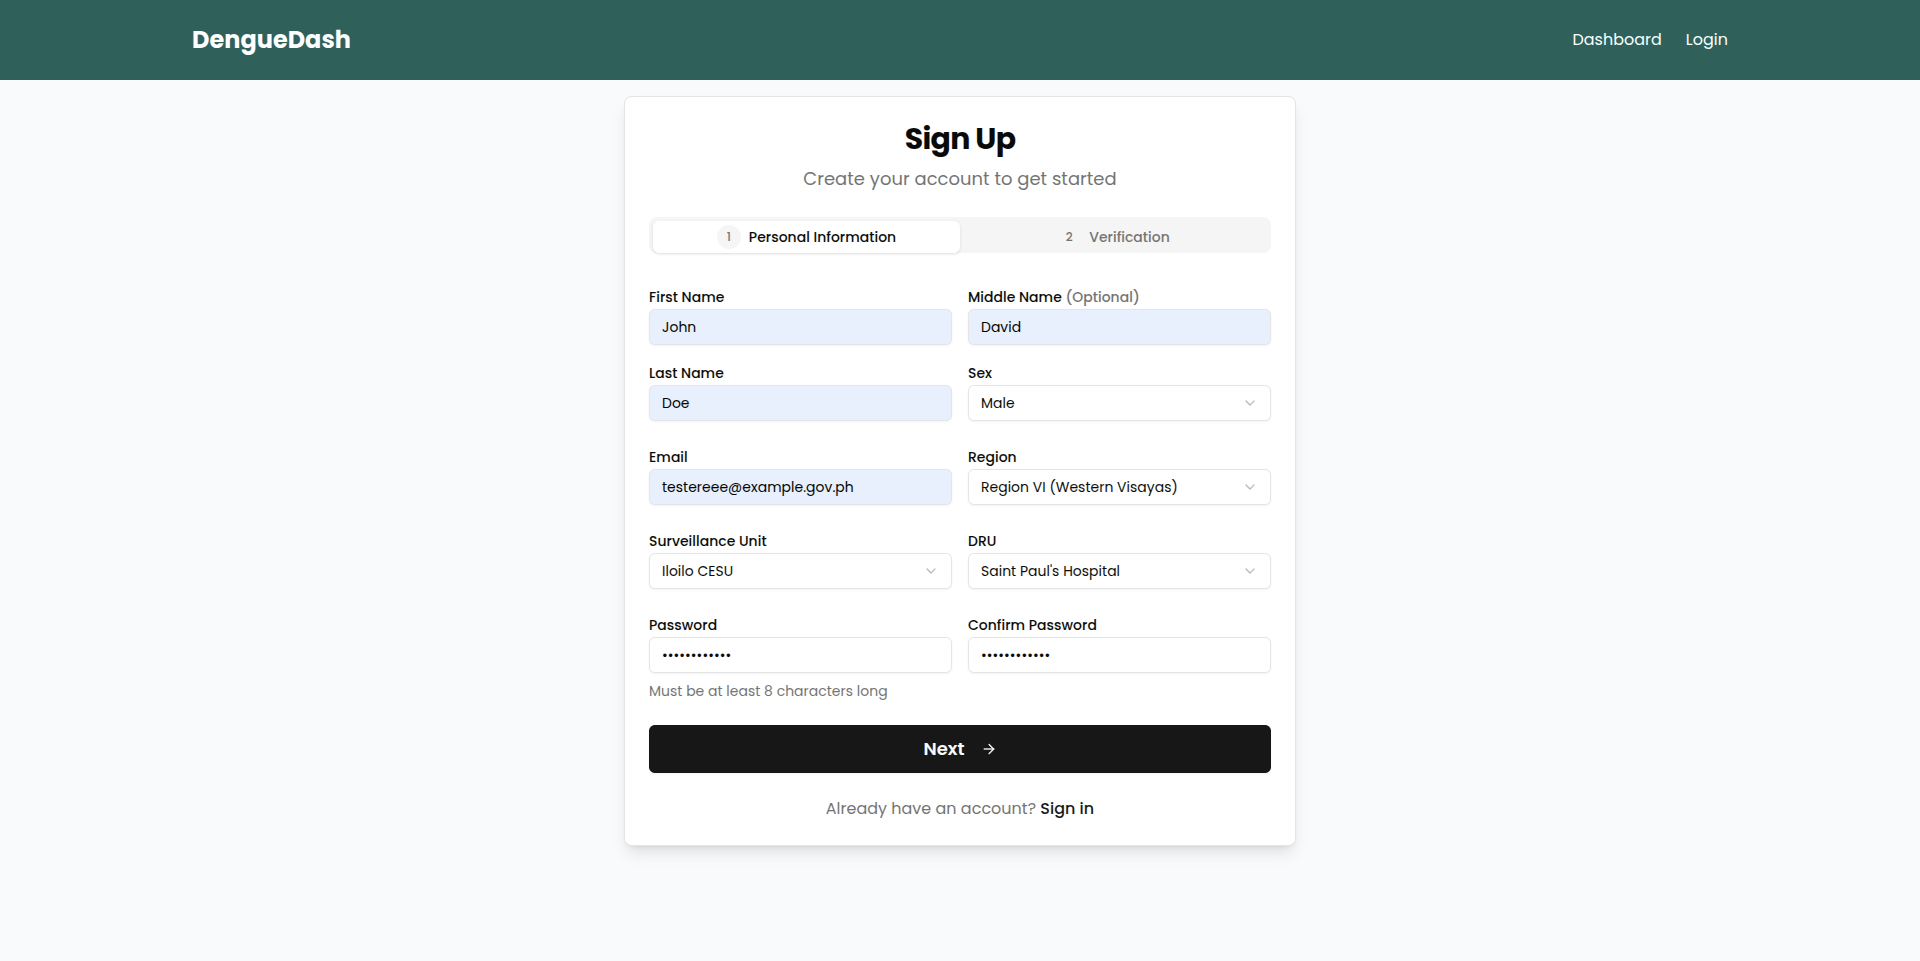
\includegraphics[width=0.8\textwidth]{signup_page_1}
	\caption{Personal Information Tab of Sign Up Page}
	\label{fig:signup_page_1}
\end{figure}
\begin{figure}[H]
	\centering
	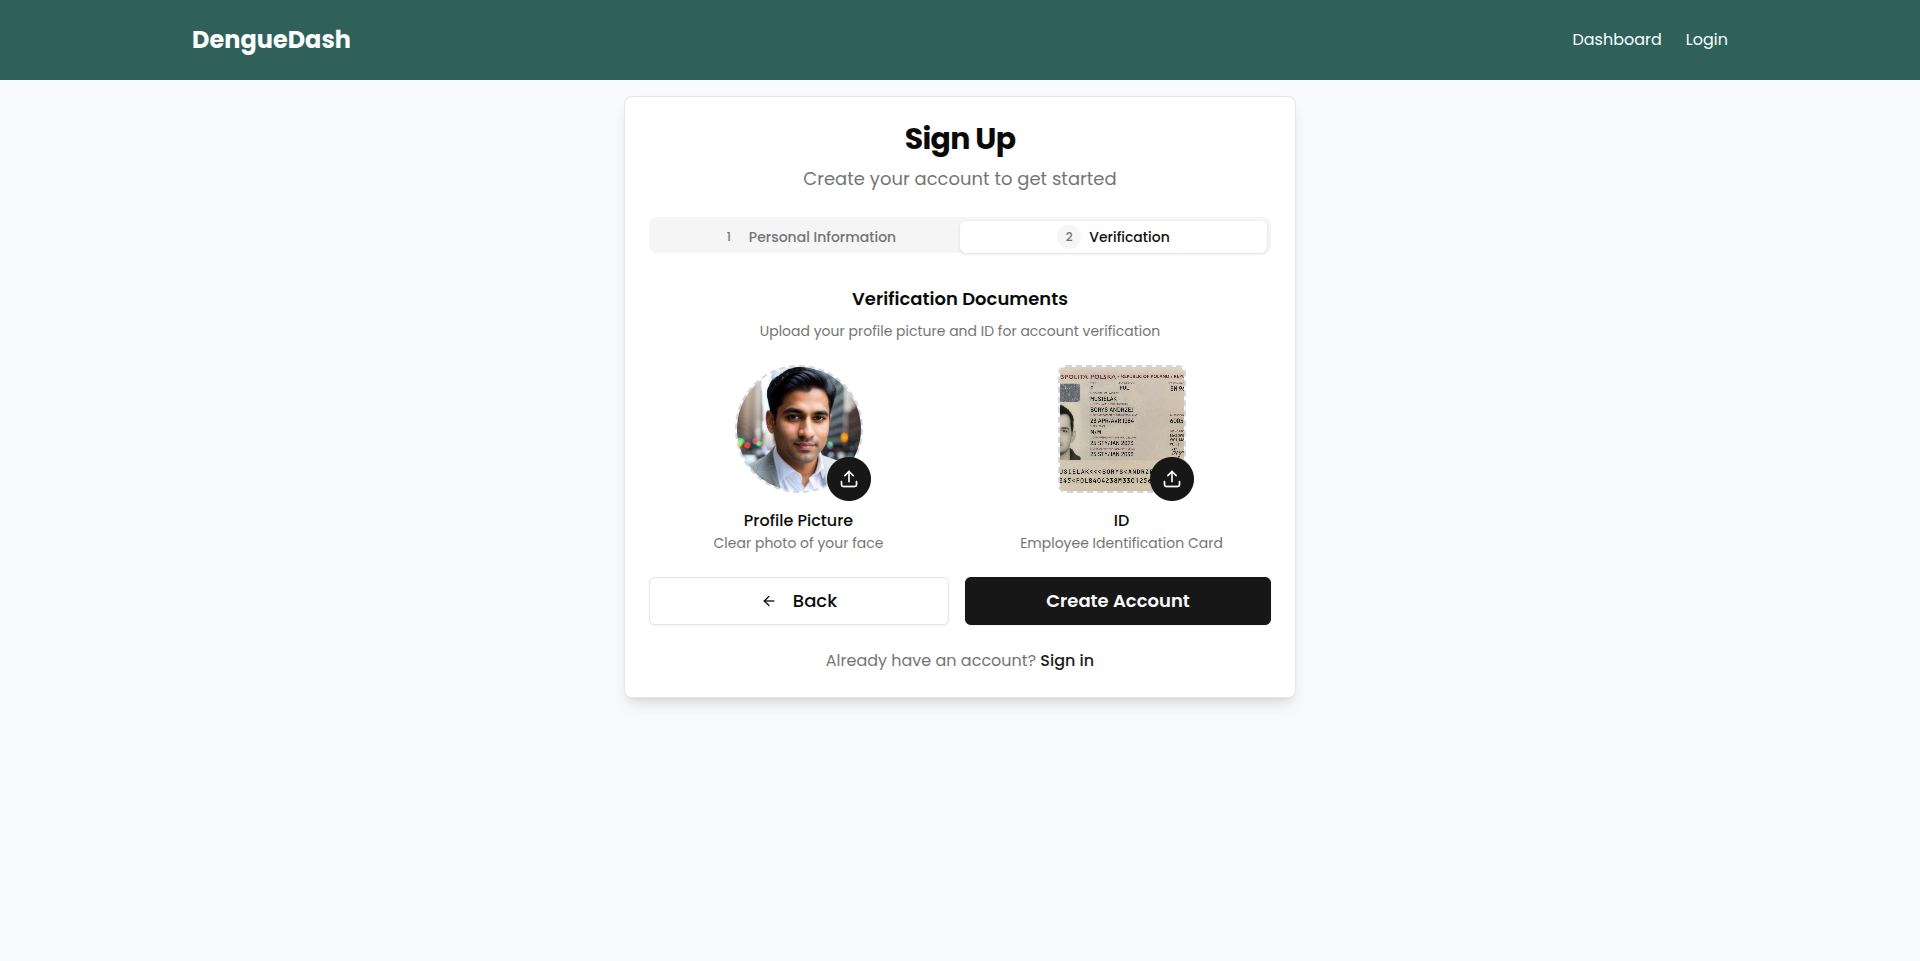
\includegraphics[width=1\textwidth]{signup_page_2}
	\caption{Verification Tab of Sign Up Page}
	\label{fig:signup_page_2}
\end{figure}

\begin{figure}[H]
	\centering
	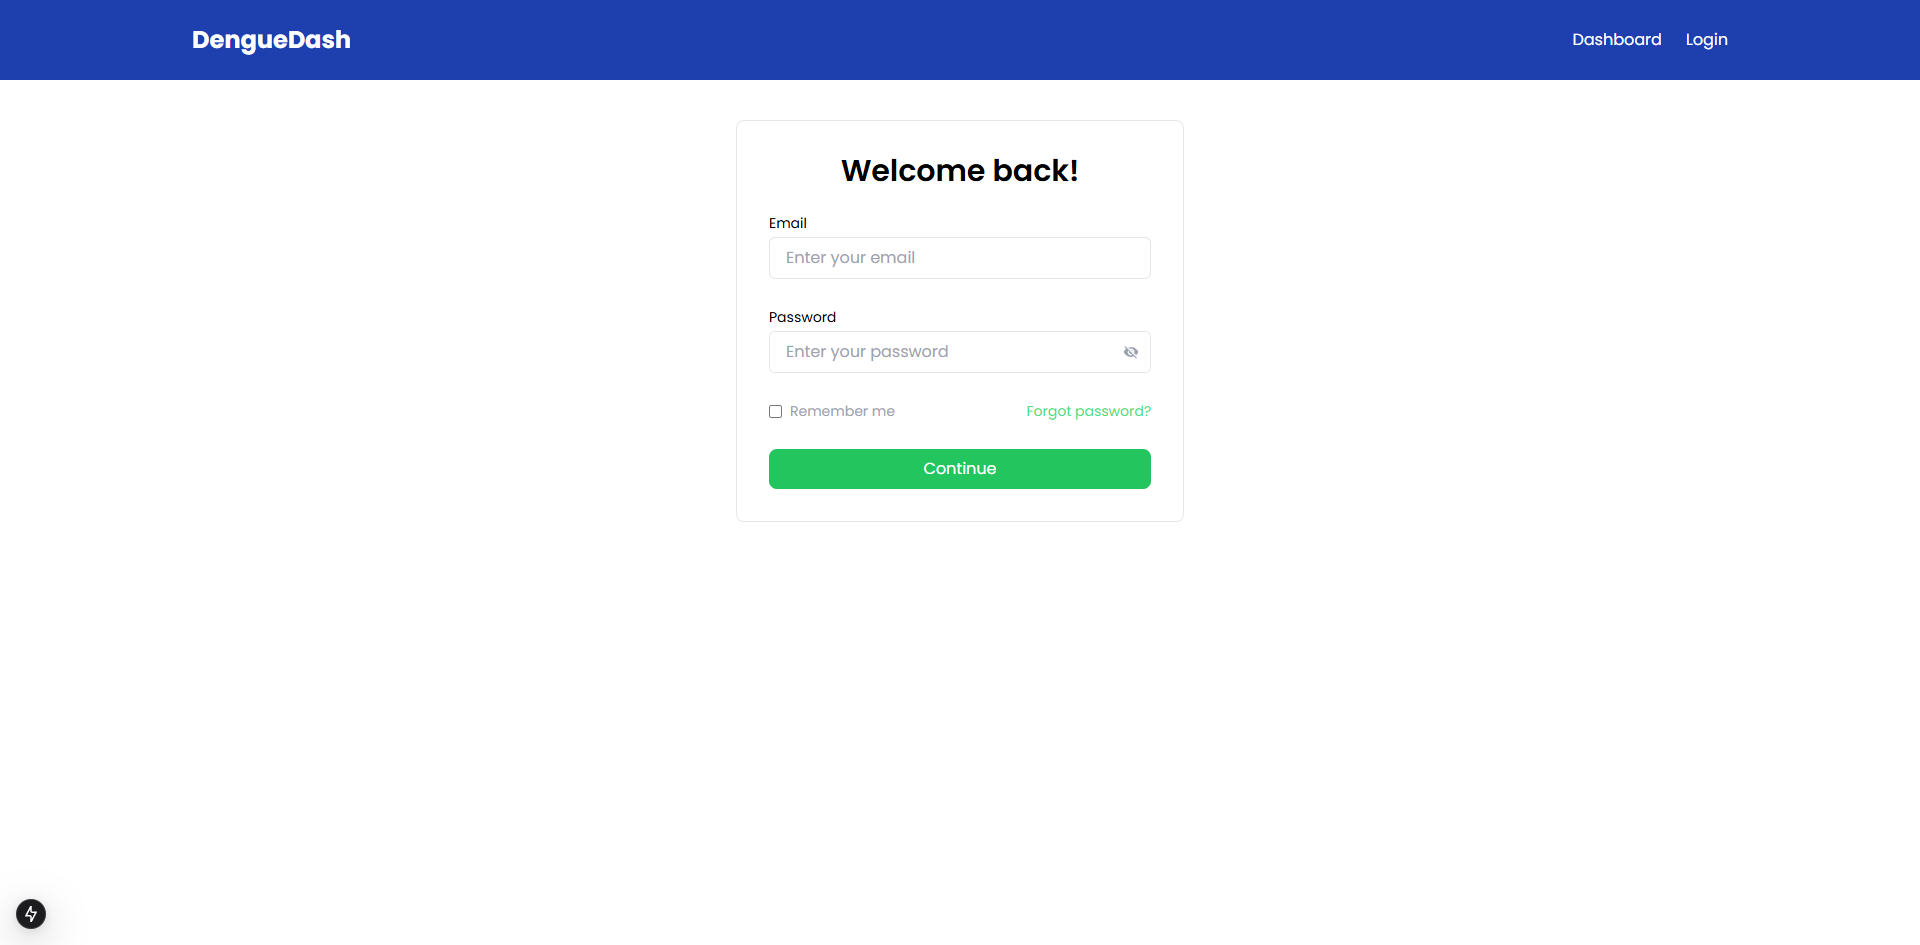
\includegraphics[width=1\textwidth]{login_page}
	\caption{Login Page}
	\label{fig:login_page}
\end{figure}

\subsection{Encoder Interface}
\subsubsection{Case Report Form}
Figures \ref{fig:case_report_form_1} and \ref{fig:case_report_form_2} show the digitized counterpart of the form obtained from the Iloilo Provincial Epidemiology and Surveillance Unit. As the system aims to support expandability for future features, some fields were modified to accommodate more detailed input. It is worth noting that all of the included fields adhere to the latest Philippine Integrated Disease and Surveillance Response (PIDSR) Dengue Forms, which the referenced form was based on. By doing this, if implemented on a national scale, the transition between targeted users will be easier. Moreover, the case form includes the patient's basic information, dengue vaccination status, consultation details, laboratory results, and the outcome. On the other hand, encoders can also create case records using a "bulk upload" feature that makes use of a formatted CSV file template. As shown in Figure \ref{fig:bulk_upload}, an encoder can download the template using the "Download Template" button, and insert multiple records inside the file, then upload it by clicking the "Click to upload" button. The web application automatically checks the file for data inconsistencies and validation. 

\begin{figure}[H]
	\centering
	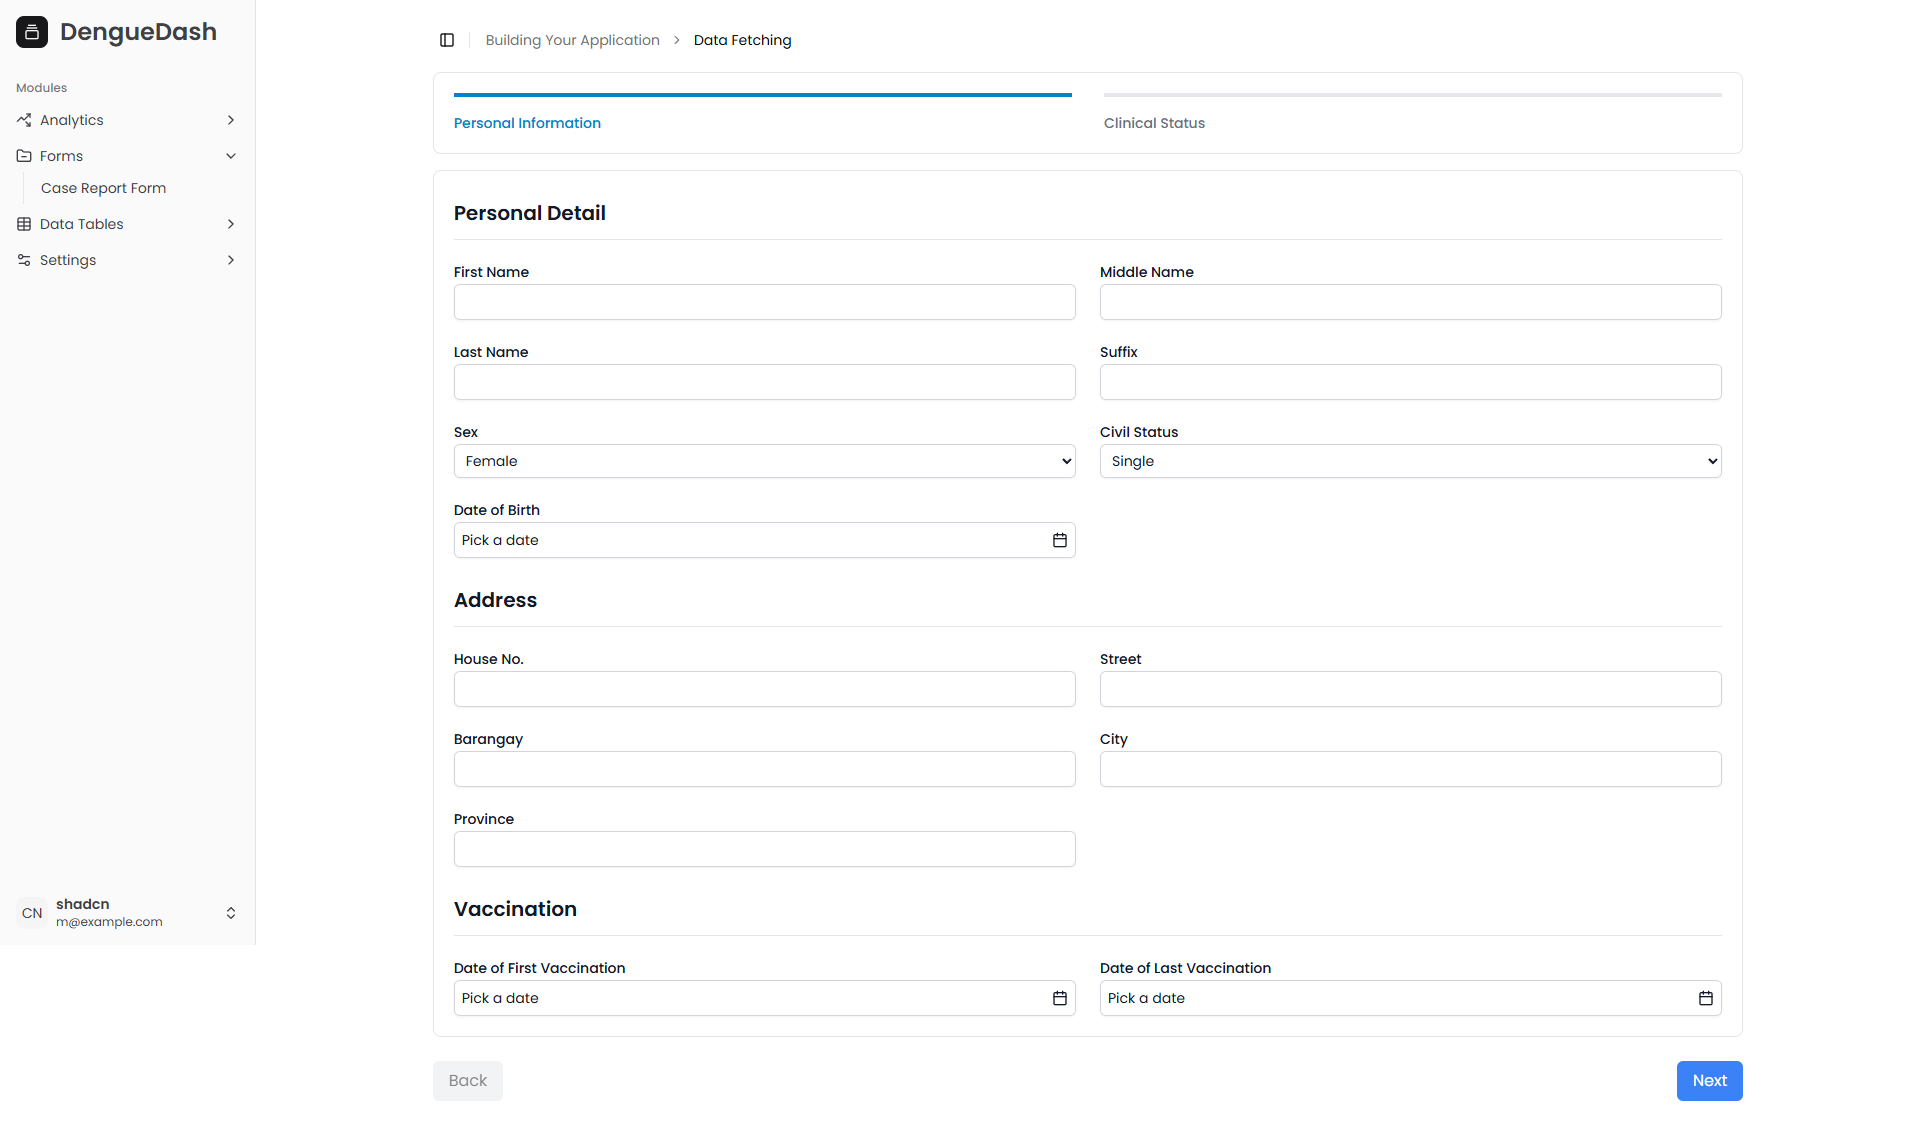
\includegraphics[width=0.8\textwidth]{case_report_form_1}
	\caption{First Part of Case Report Form}
	\label{fig:case_report_form_1}
\end{figure}
\begin{figure}[H]
	\centering
	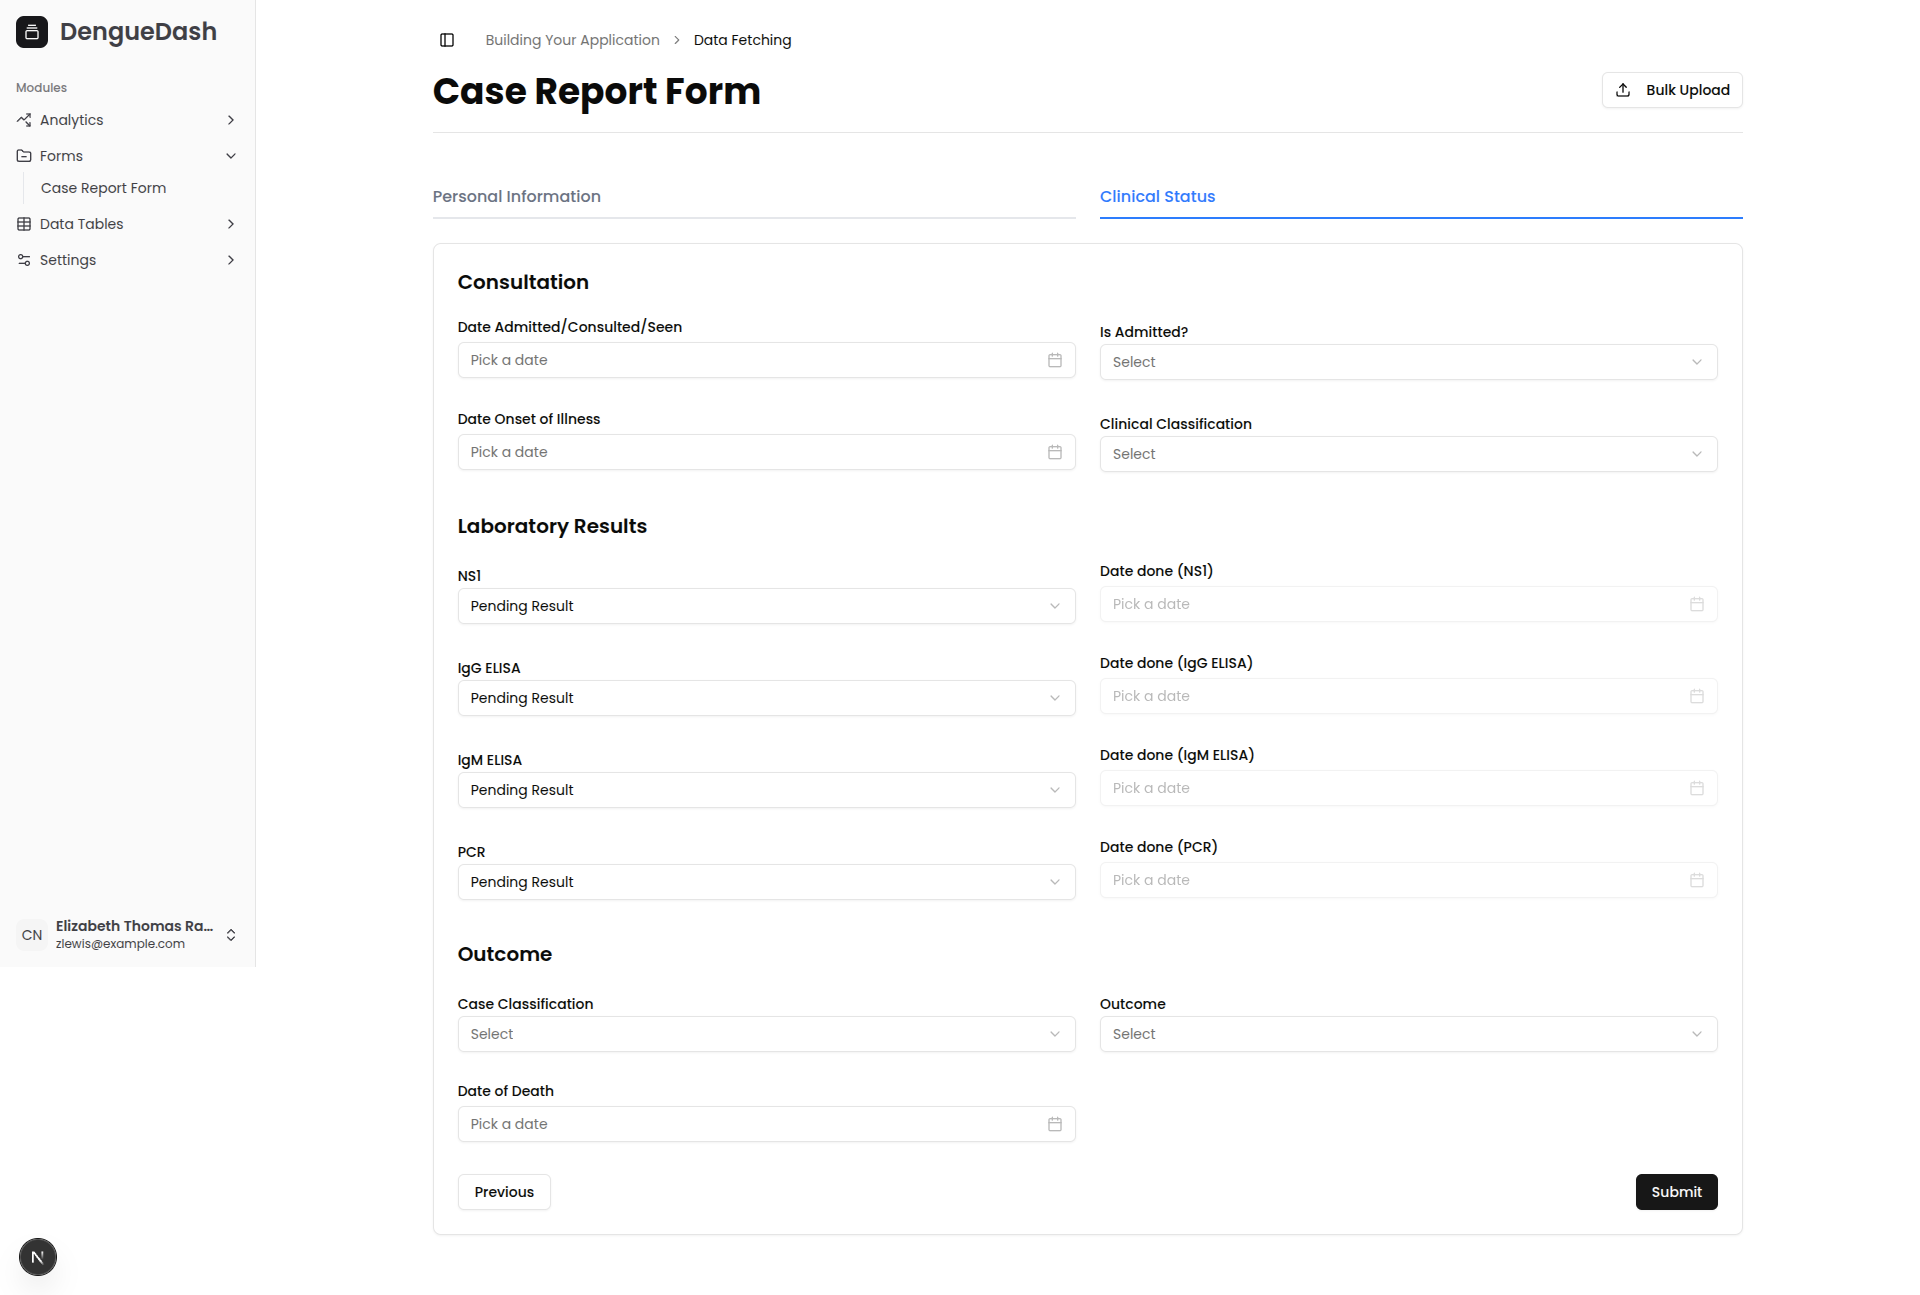
\includegraphics[width=0.8\textwidth]{case_report_form_2}
	\caption{Second Part of Case Report Form}
	\label{fig:case_report_form_2}
\end{figure}

\begin{figure}[H]
	\centering
	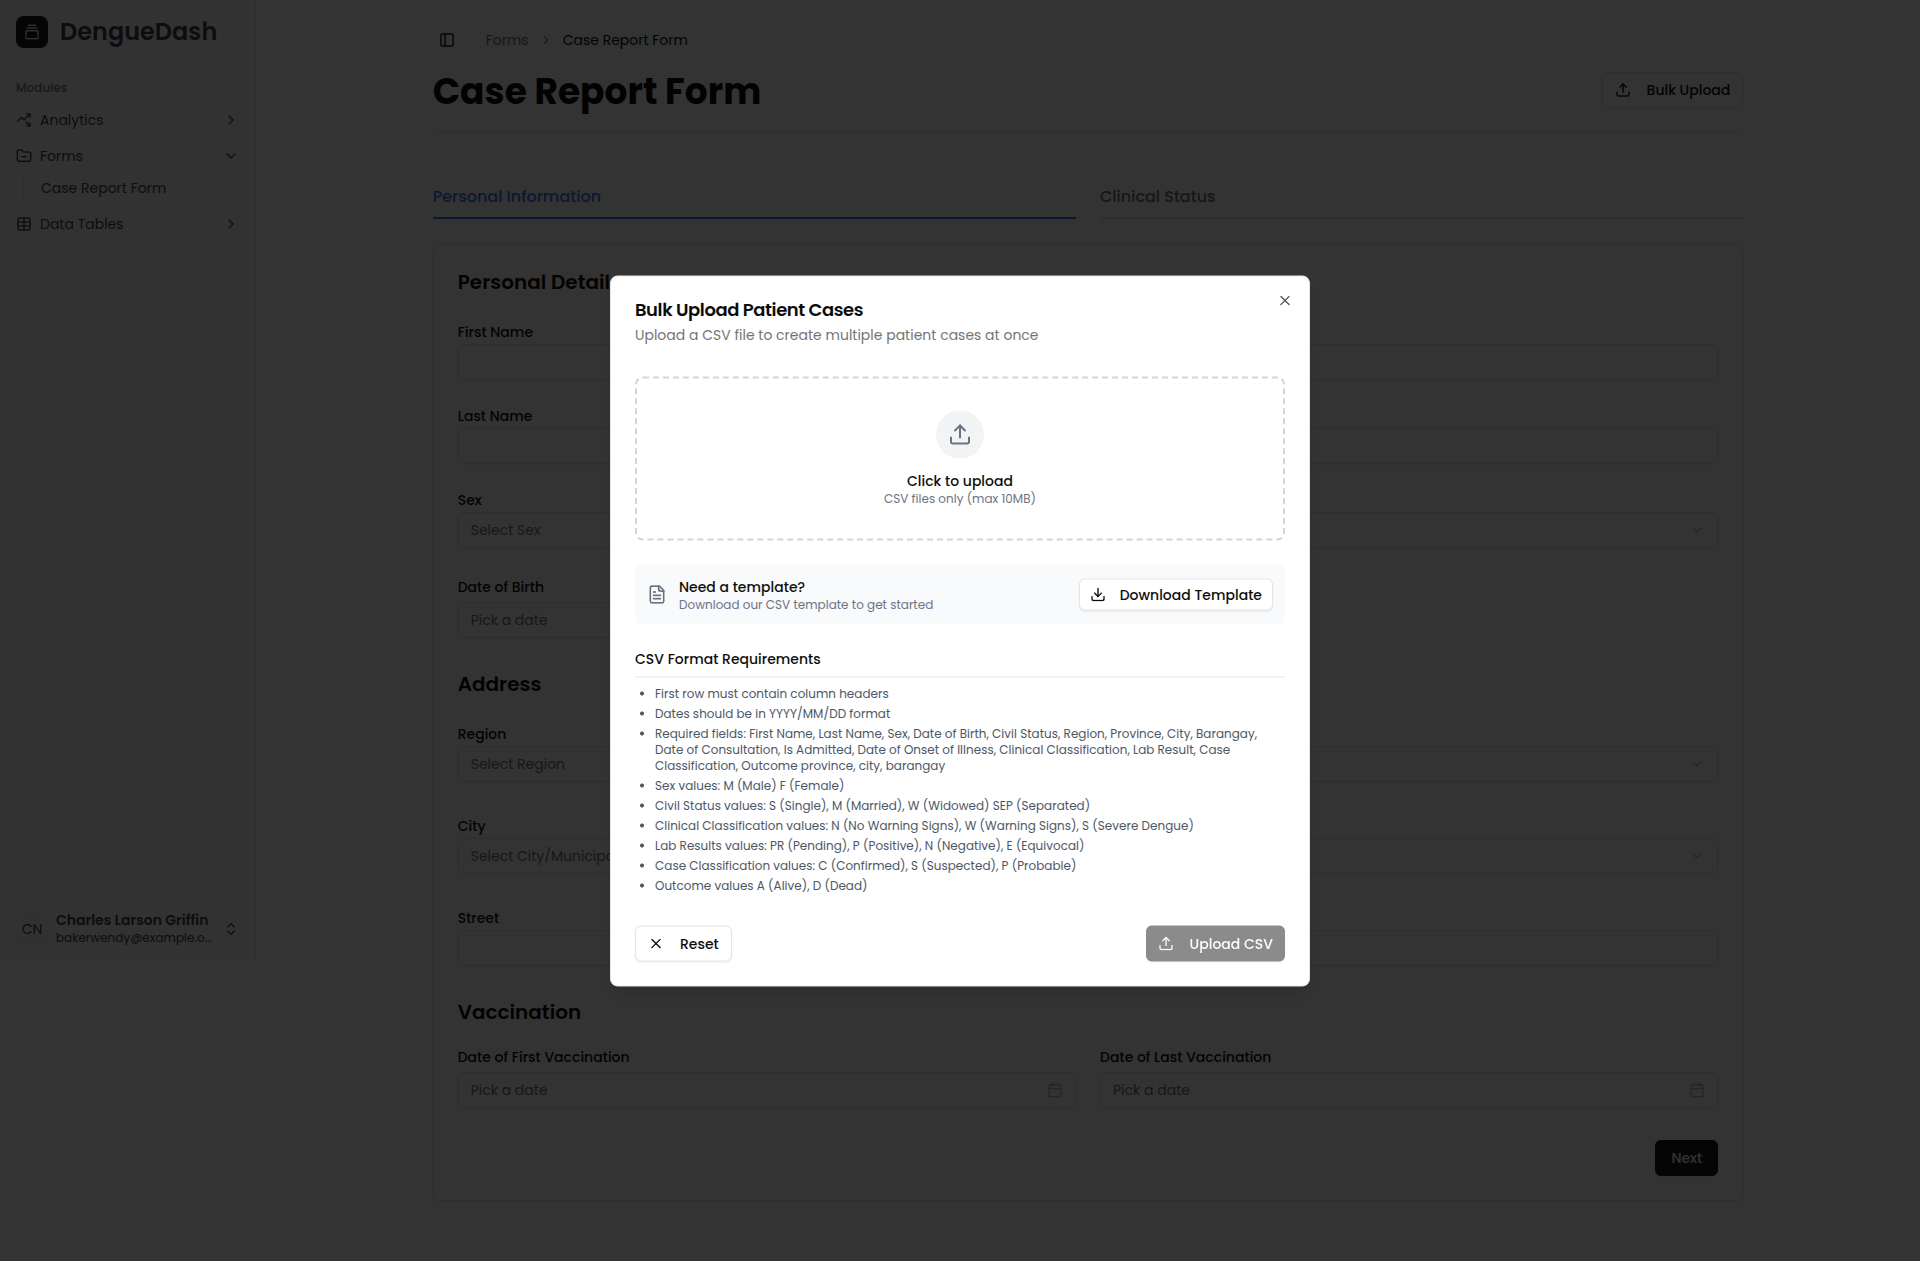
\includegraphics[width=1\textwidth]{bulk_upload}
	\caption{Bulk Upload of Cases using CSV}
	\label{fig:bulk_upload}
\end{figure}

\subsubsection{Browsing, Update, and Deletion of Records}
Once the data generated from the case report form or the bulk upload is validated, it will be assigned as a new case and can be accessed through the Dengue Reports page, as shown in Figure \ref{fig:dengue_reports}. The said page displays basic information about the patient related to a specific case, including their name, address, date of consultation, and clinical and case classifications. It is also worth noting that it only shows cases that the user is permitted to view. For example, in a local Disease Reporting Unit (DRU) setting, the user can only access records that belong to the same DRU. Additionally, users can search for cases by name, location, date of consultation, or classifications associated with the specific query, making it easier to find pertinent information quickly and efficiently. On the other hand, in a consolidated surveillance unit such as a regional, provincial, or city quarter, its users can view all the records from all the DRUs that report to them. Moving forward, Figure \ref{fig:detailed_case_report} shows the detailed case report of the patient on a particular consultation date. 

\begin{figure}[H]
	\centering
	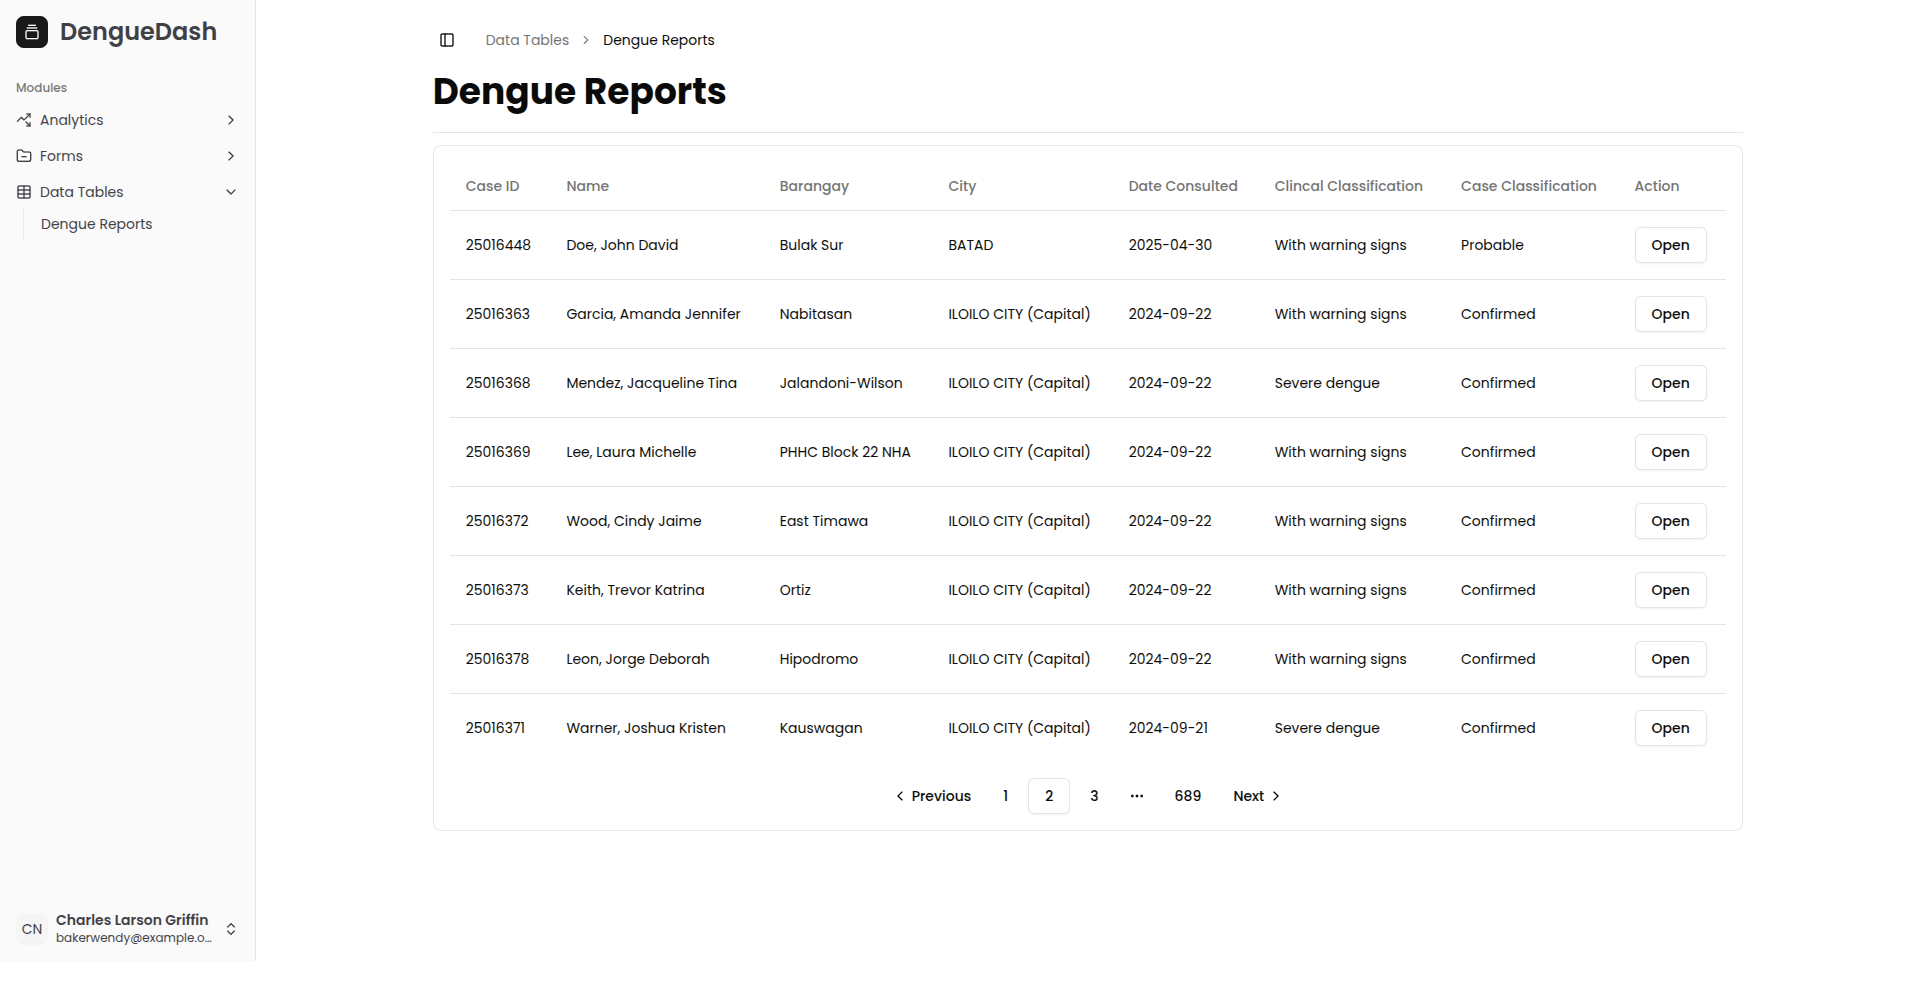
\includegraphics[width=1\textwidth]{dengue_reports}
	\caption{Dengue Reports}
	\label{fig:dengue_reports}
\end{figure}
\begin{figure}[H]
	\centering
	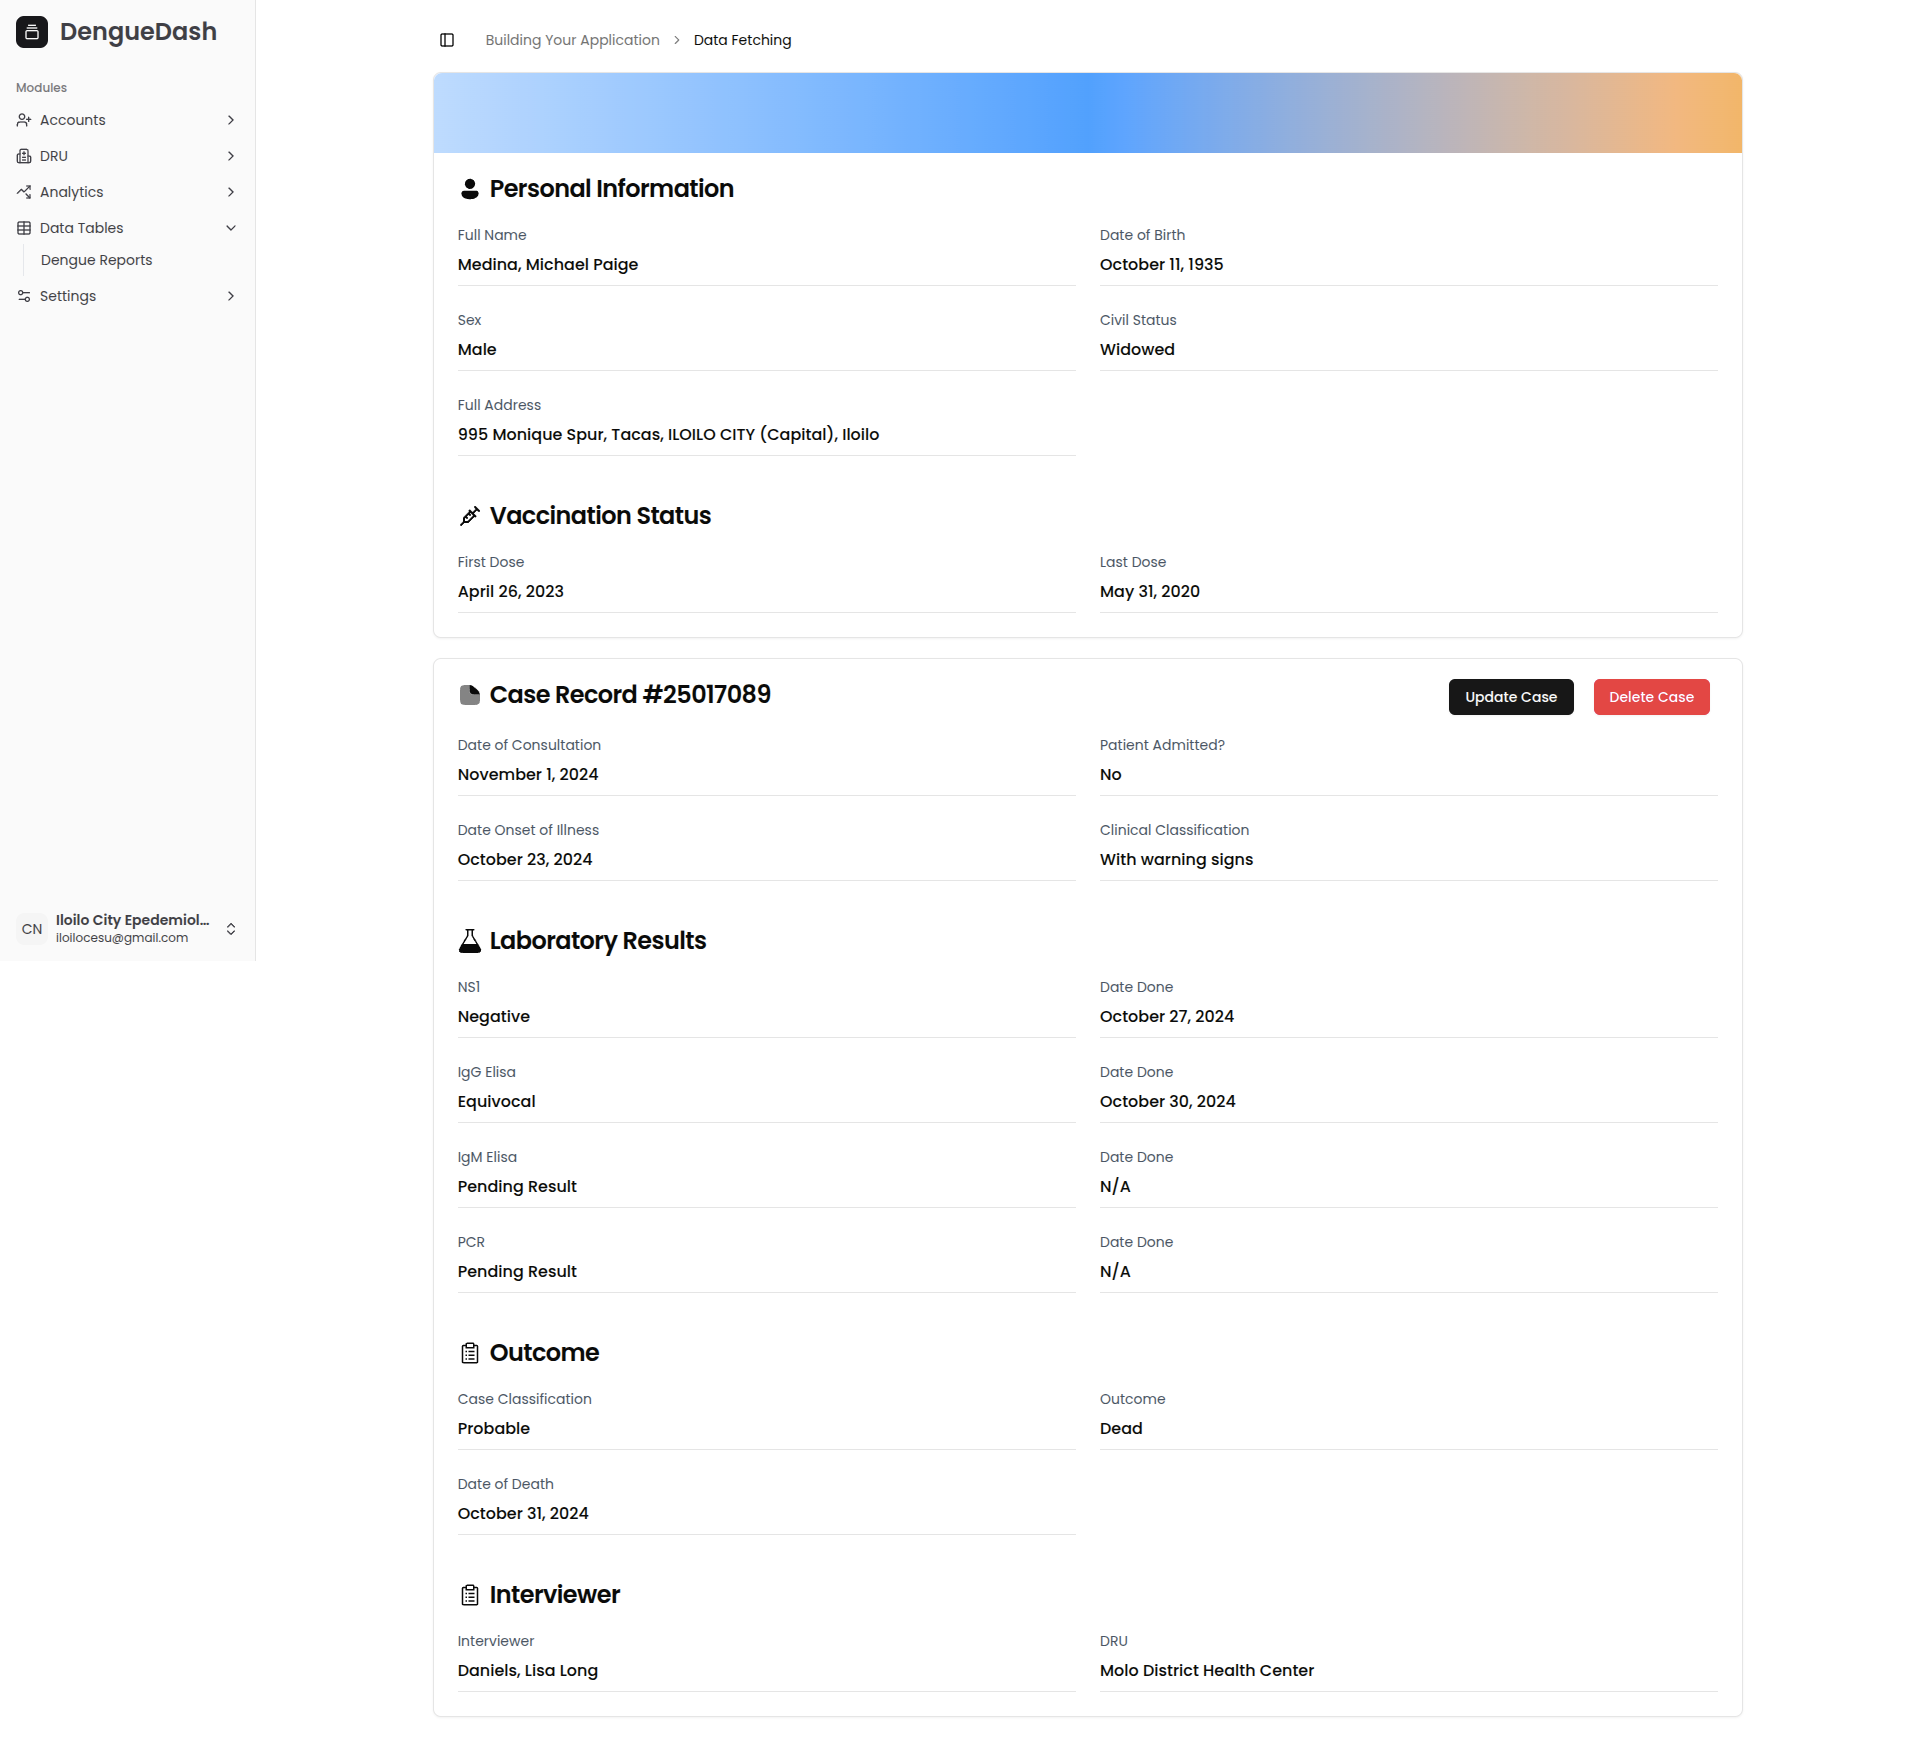
\includegraphics[width=1\textwidth]{detailed_case_report}
	\caption{Detailed Case Report}
	\label{fig:detailed_case_report}
\end{figure}

To update the case, the user can click the "Update Case" button, where a dialog will appear, and the updateable fields will be shown. It is worth noting that in this case, only fields under Laboratory Results and Outcome are included since they are the only ones that are time-based, where the result may change in the future. After updating, a prompt will show confirming the user's action. Moving forward, to delete a case record, the user must click the "Delete Case" button, and a prompt verifying the action will appear. After confirming, the case will be deleted permanently.

\begin{figure}[H]
	\centering
	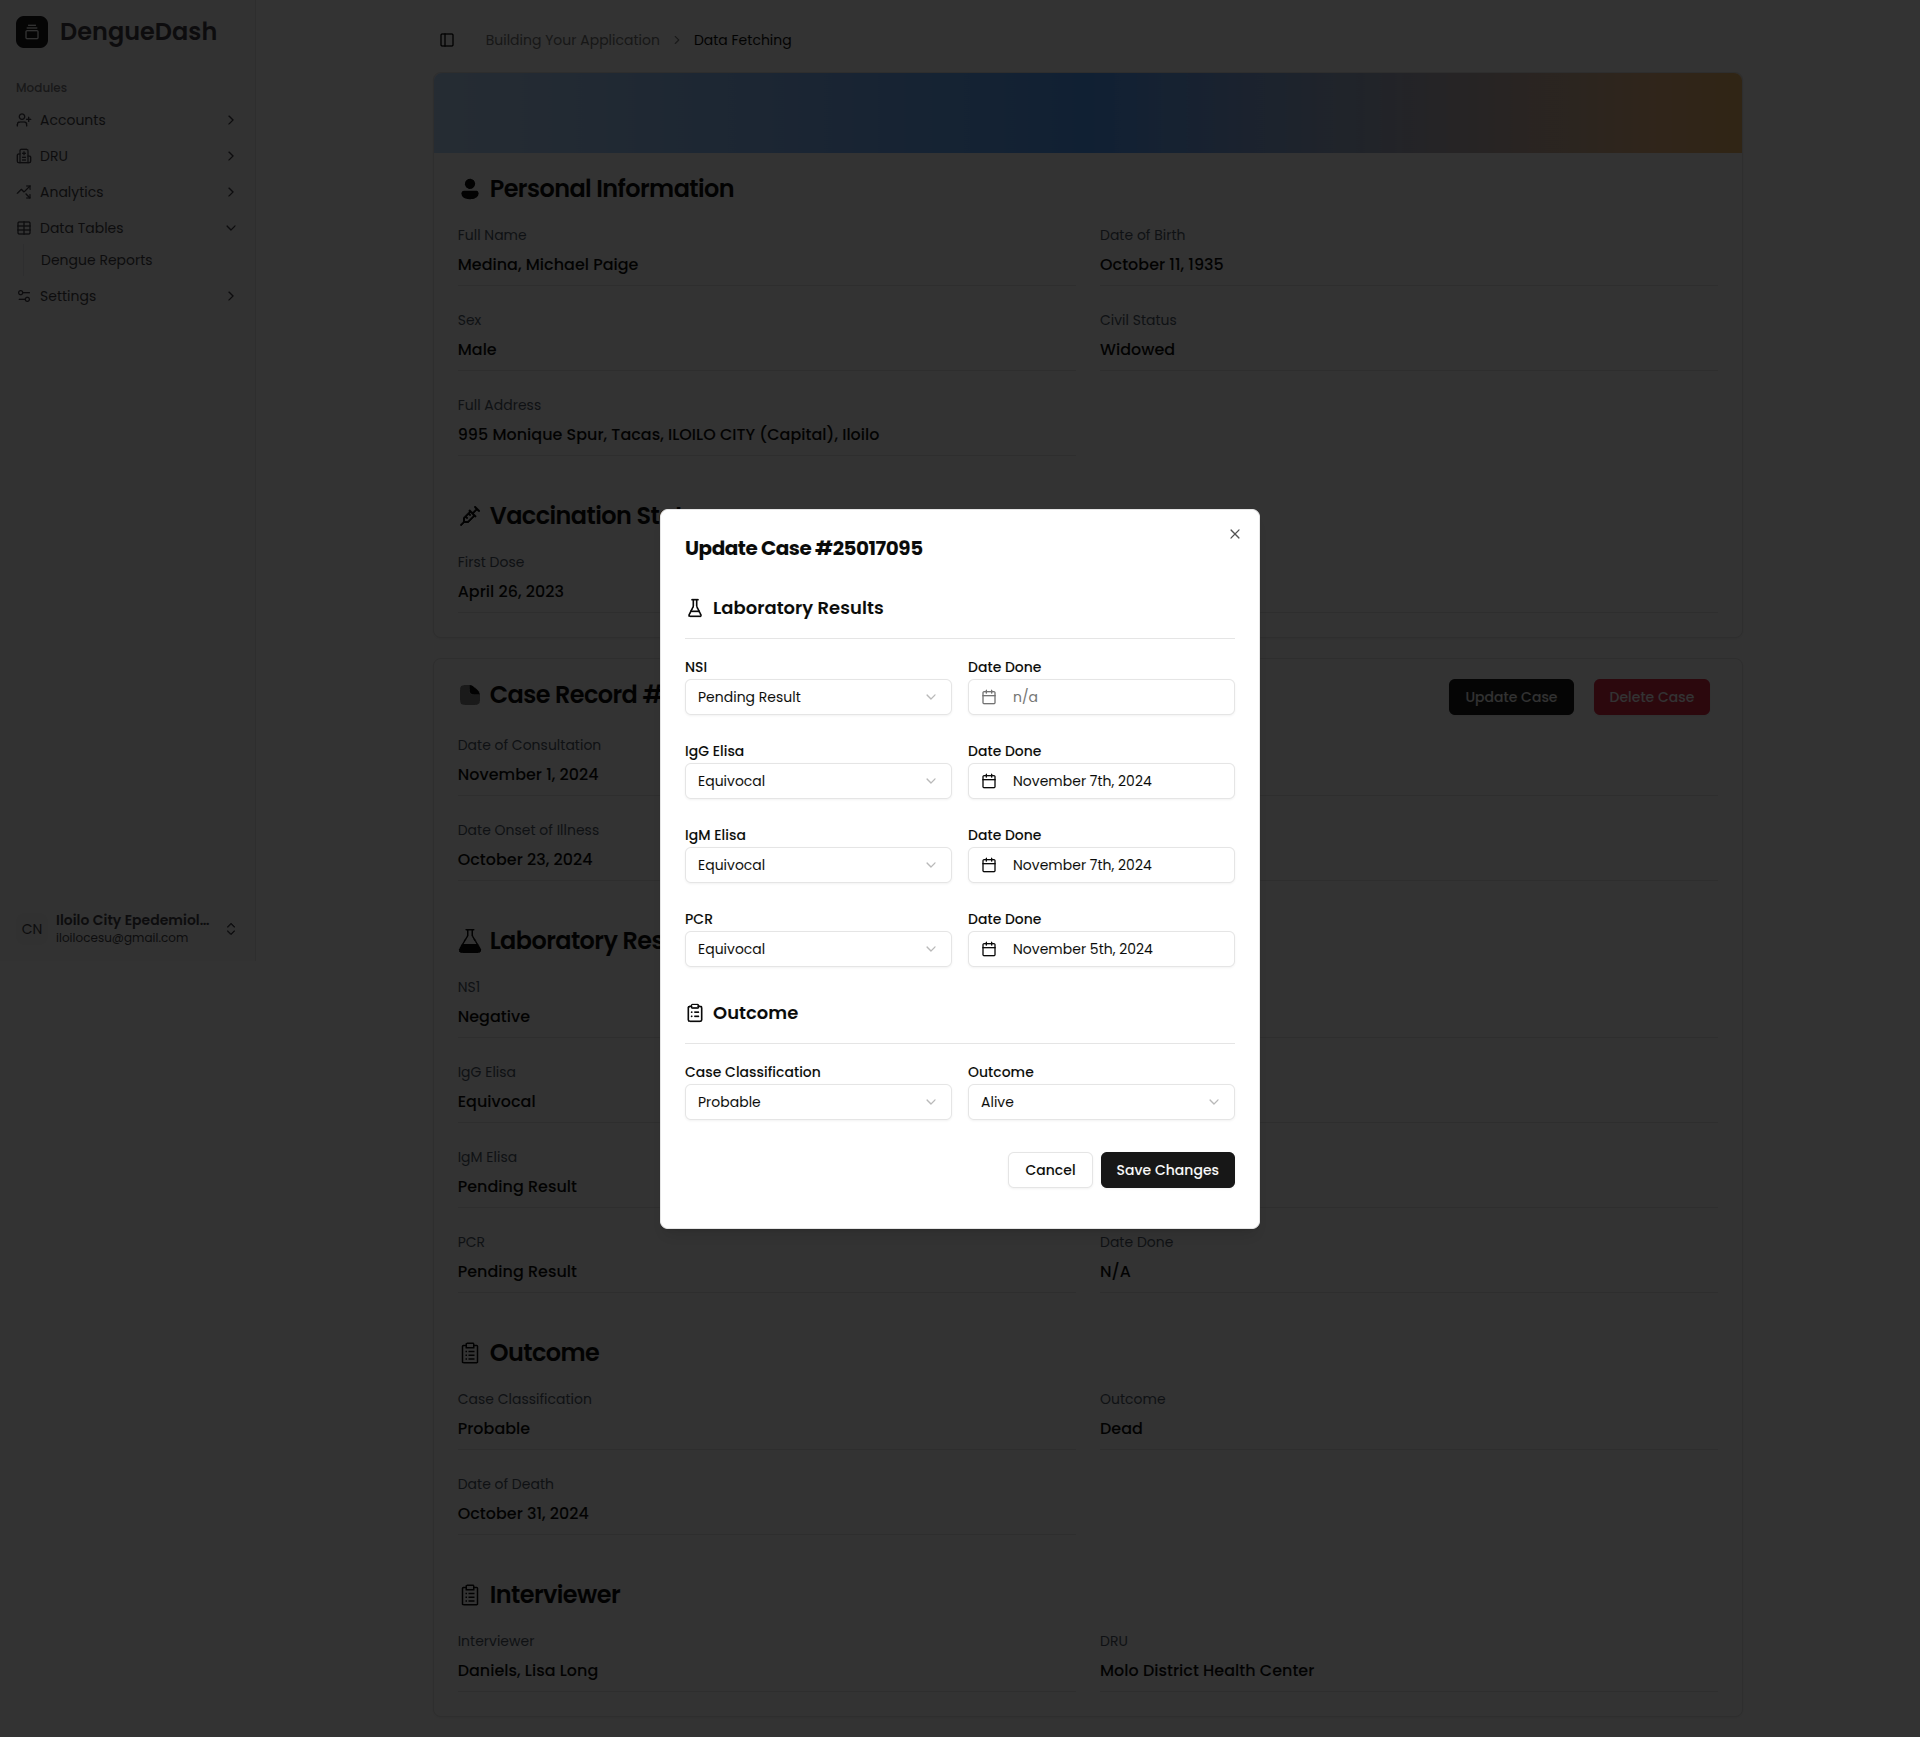
\includegraphics[width=1\textwidth]{update_report}
	\caption{Update Report Dialog}
	\label{fig:update_report}
\end{figure}
\begin{figure}[H]
	\centering
	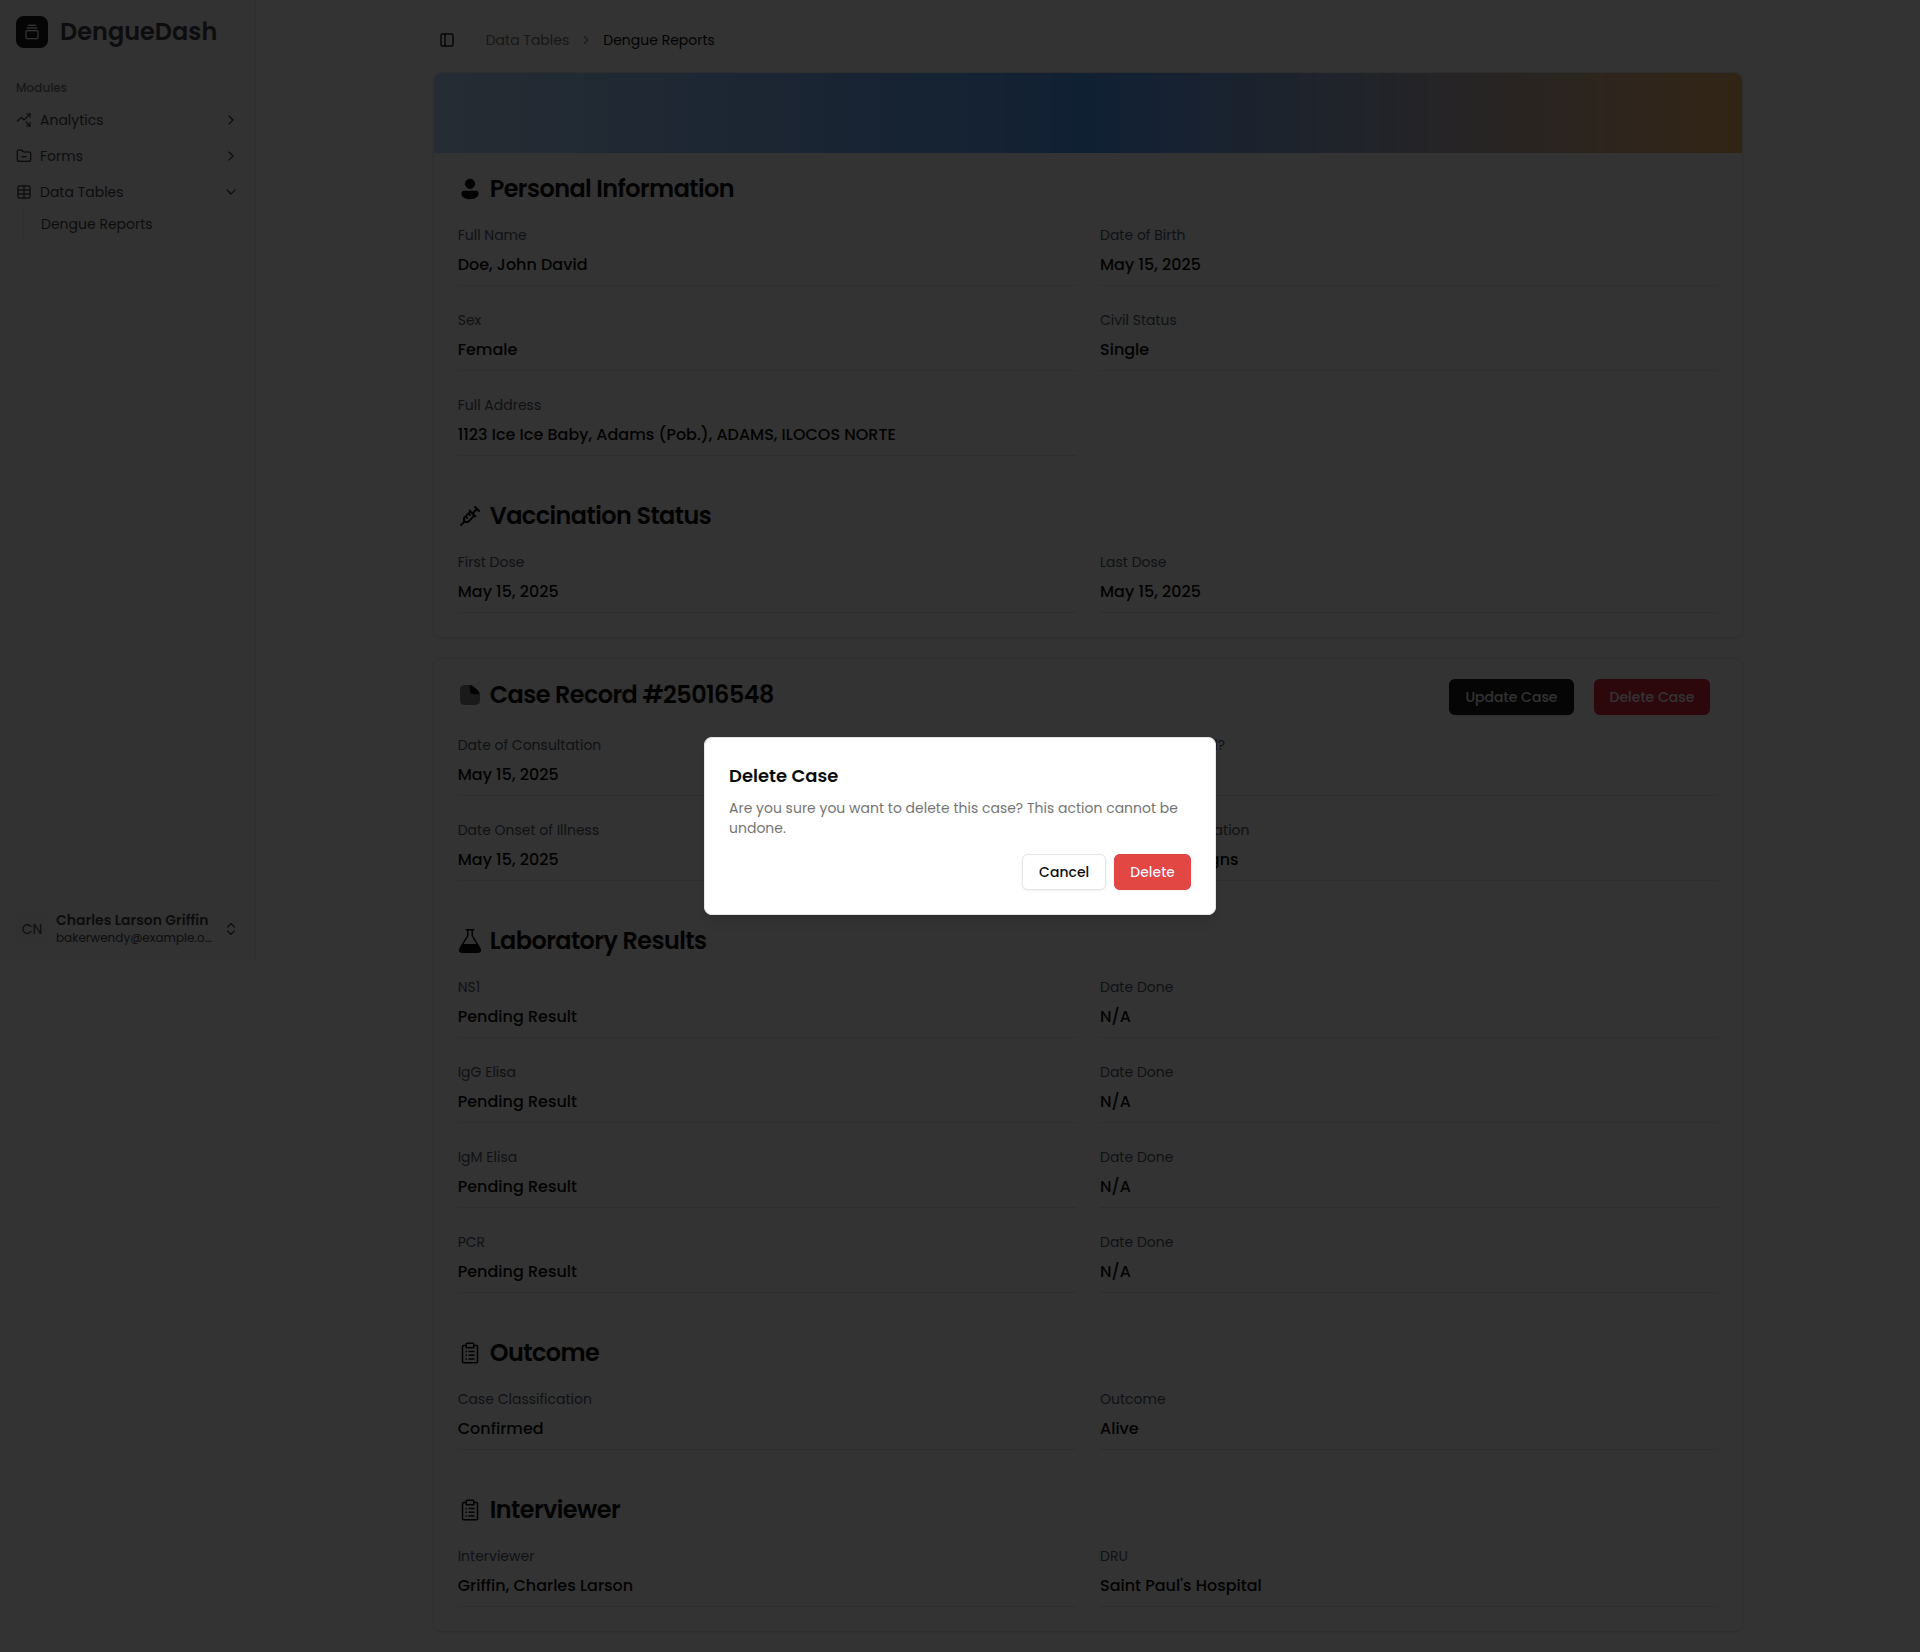
\includegraphics[width=1\textwidth]{delete_report}
	\caption{Delete Report Alert Dialog}
	\label{fig:delete_report}
\end{figure}

\subsubsection{Forecasting}

The pièce de résistance of the web application's features is the Forecasting Page. This is where users can forecast dengue cases for the next few weeks. To predict, the application utilizes the exported LSTM model in a Keras format derived from training the consolidated data from the database. The said file stores the model's architecture and the learned parameters, which include the weights and biases to predict cases without training the data again.  Furthermore, it requires the recent weekly dengue cases and weather variable data (temperature, humidity, and rainfall) to form a sequence based on the window size, and the forecasted weather data via OpenWeatherAPI. Due to the limitations posed to the current subscribed student plan in the said API, only two weeks of forecasted weather data can be fetched. As a result, the web application can predict dengue cases for the next two following weeks. Moving forward, the Forecasting page, as shown in Figure \ref{fig:forecasting}, introduces a user-friendly interface that shows the current cases for the week and the predictions for the next two weeks with a range of 90 percent to 110 percent confidence interval that is presented in a simple but organized manner. There is also a line chart that shows the number of cases from the last 5 weeks plus the forecasted weekly cases. In addition, the current weather data for a specific week is also shown, as well as the forecasted weather data fetched from the said API. Lastly, locations where dengue cases have been reported for the current week are listed in the Location Risk Assessment component. 

\begin{figure}[H]
	\centering
	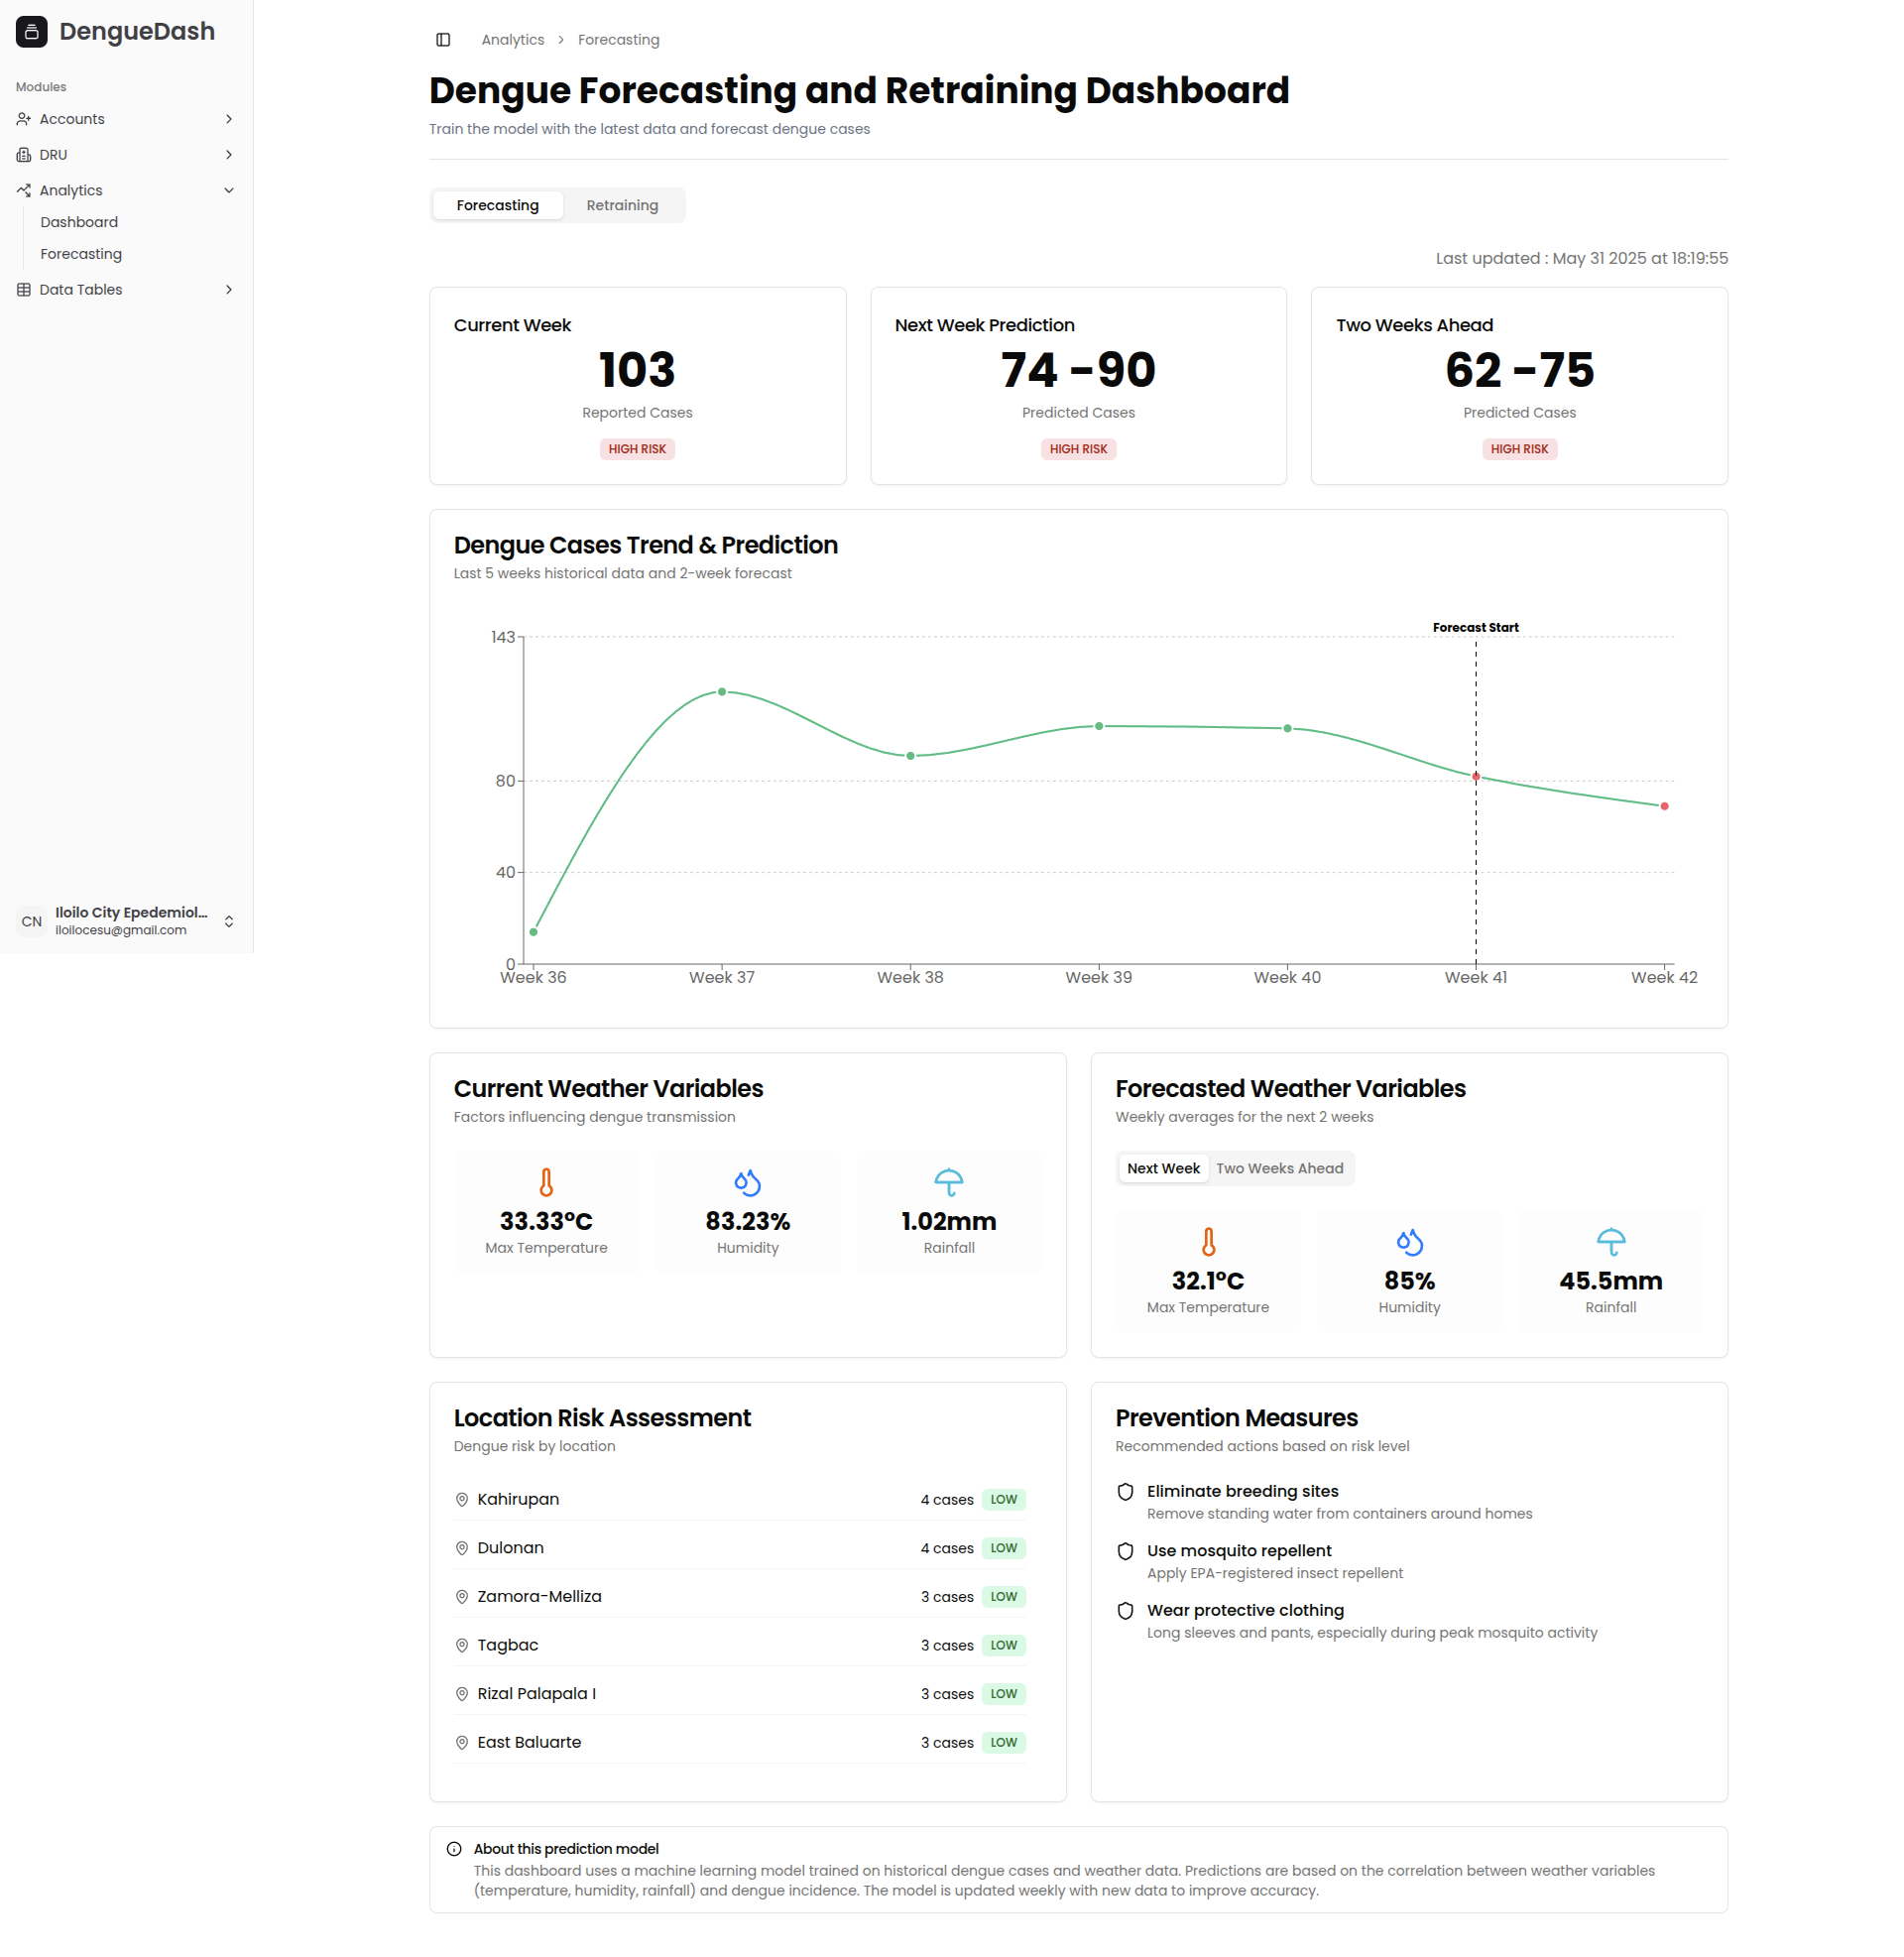
\includegraphics[width=1\textwidth]{forecasting}
	\caption{Forecasting Page}
	\label{fig:forecasting}
\end{figure}

\subsection{Admin Interface}

\subsubsection{Retraining}

With LSTM being the best-performing model among the models used in forecasting dengue cases, it is the model chosen to power the prediction and retraining of the consolidated data within the web application. Since the retraining process consumes a lot of processing power and requires a more advanced understanding of how it works, it was decided that the said feature should only be available to admin users of surveillance units. Furthermore, the retraining component in the Forecasting page includes three additional components that include the configuration of LSTM parameters (Figure \ref{fig:retraining_configs}), the actual retraining of the consolidated data from the database (Figure \ref{fig:retraining_train}), and the results of the retraining that shows the current and previous model metrics depending on the parameters entered (Figure \ref{fig:retraining_results}). It is also worth noting that when training, the model used a seeded number to promote reproducibility. 

\begin{figure}[H]
	\centering
	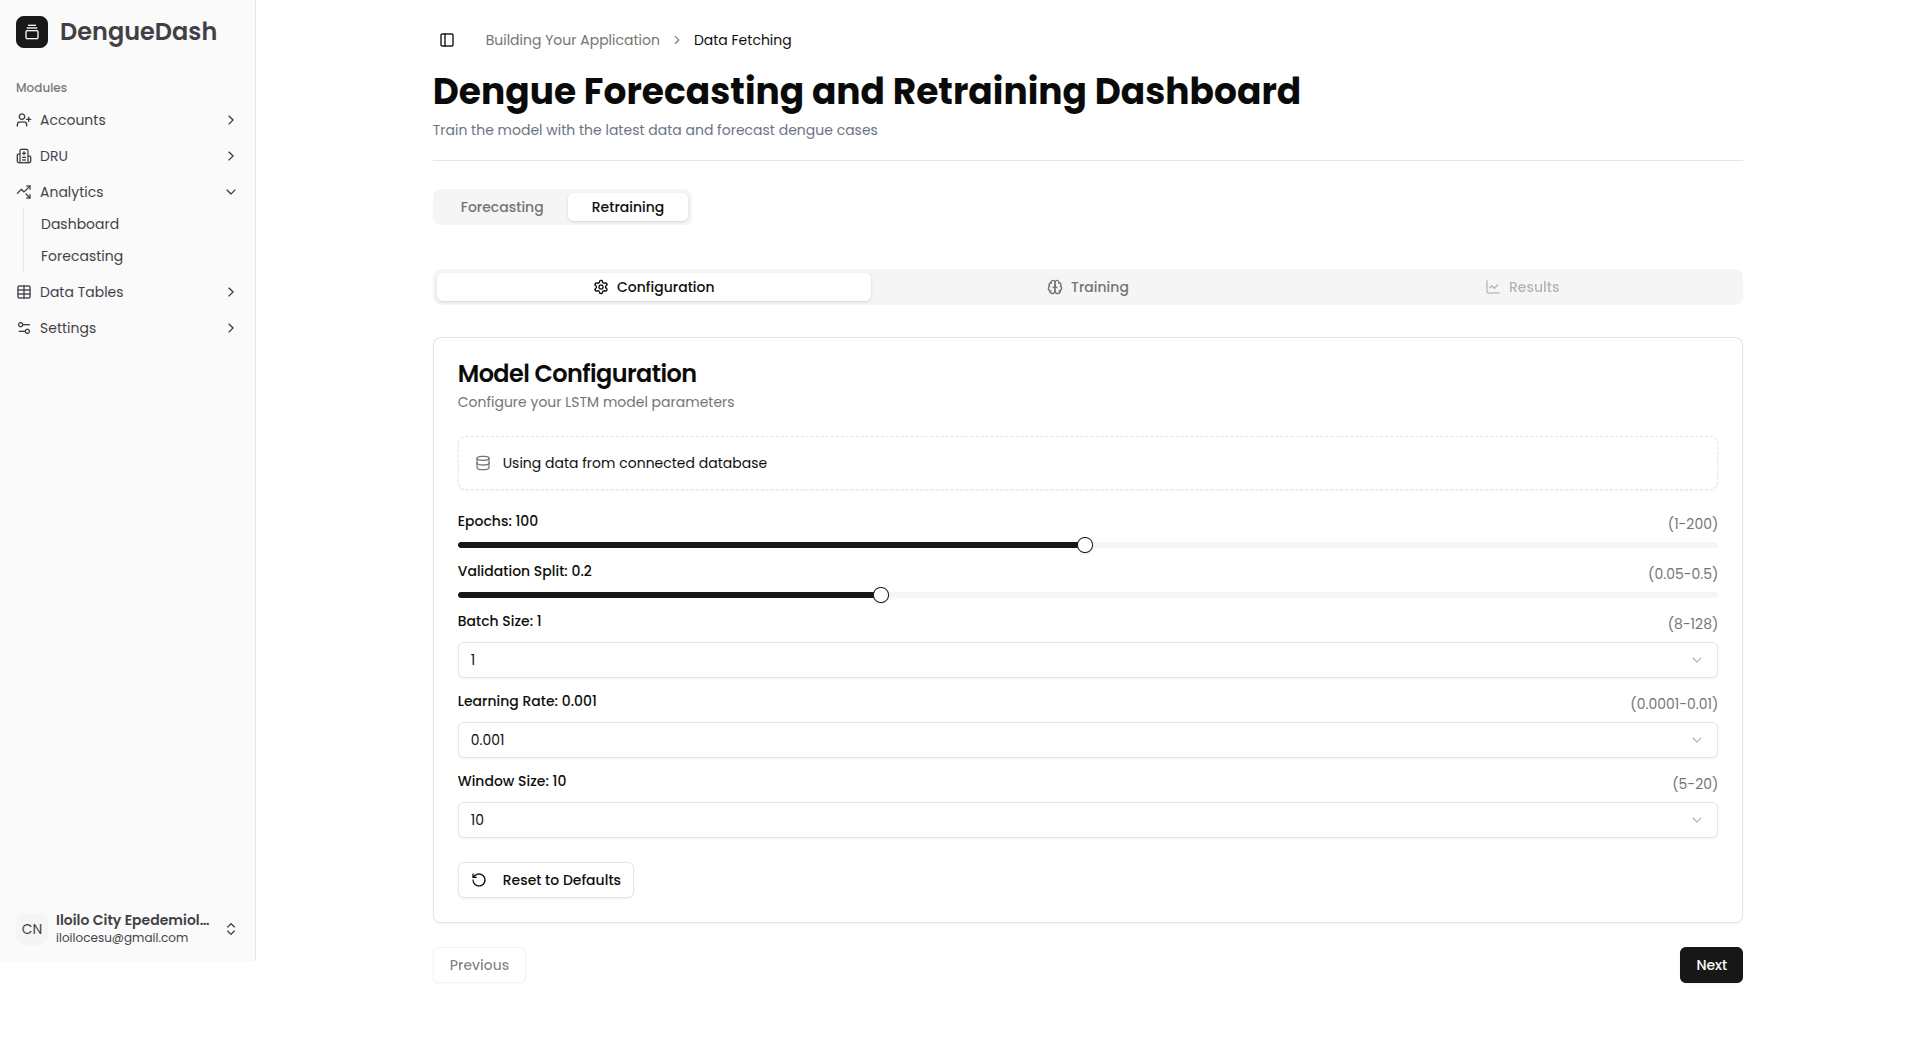
\includegraphics[width=0.8\textwidth]{retraining_configs}
	\caption{Retraining Configurations}
	\label{fig:retraining_configs}
\end{figure}
\begin{figure}[H]
	\centering
	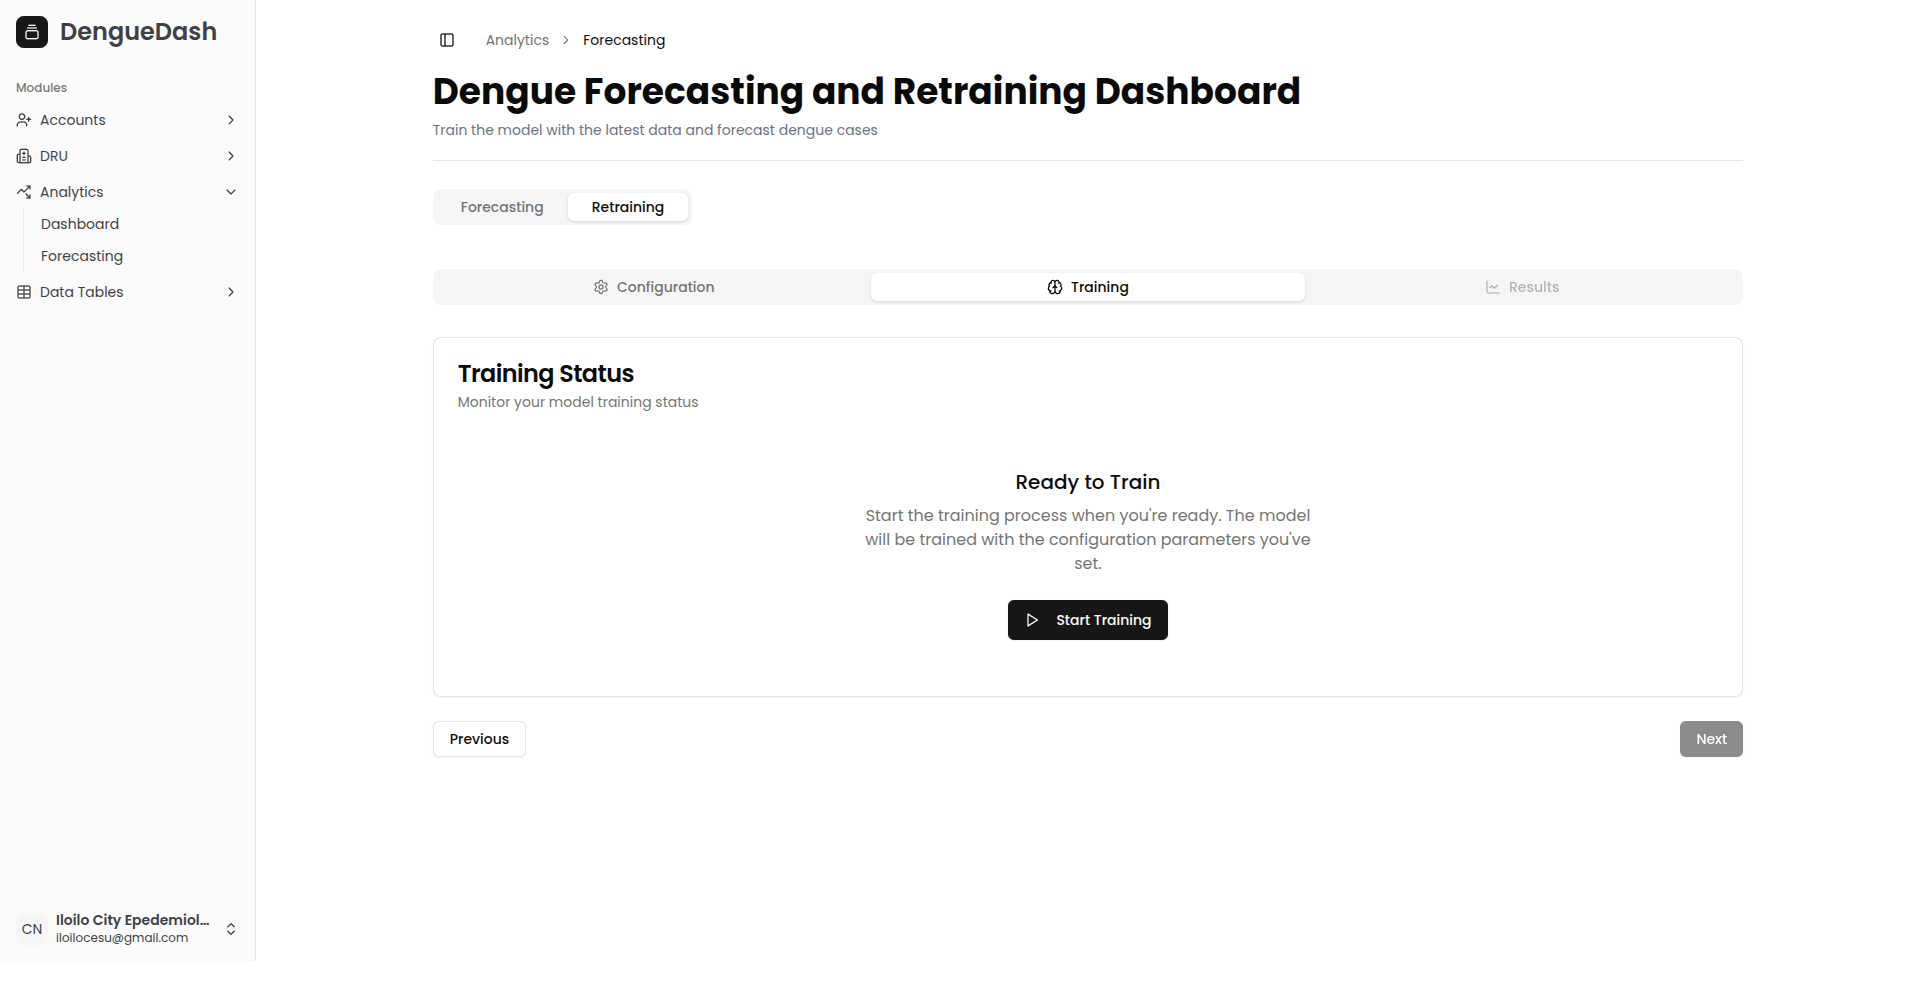
\includegraphics[width=1\textwidth]{retraining_train}
	\caption{Start Retraining}
	\label{fig:retraining_train}
\end{figure}
\begin{figure}[H]
	\centering
	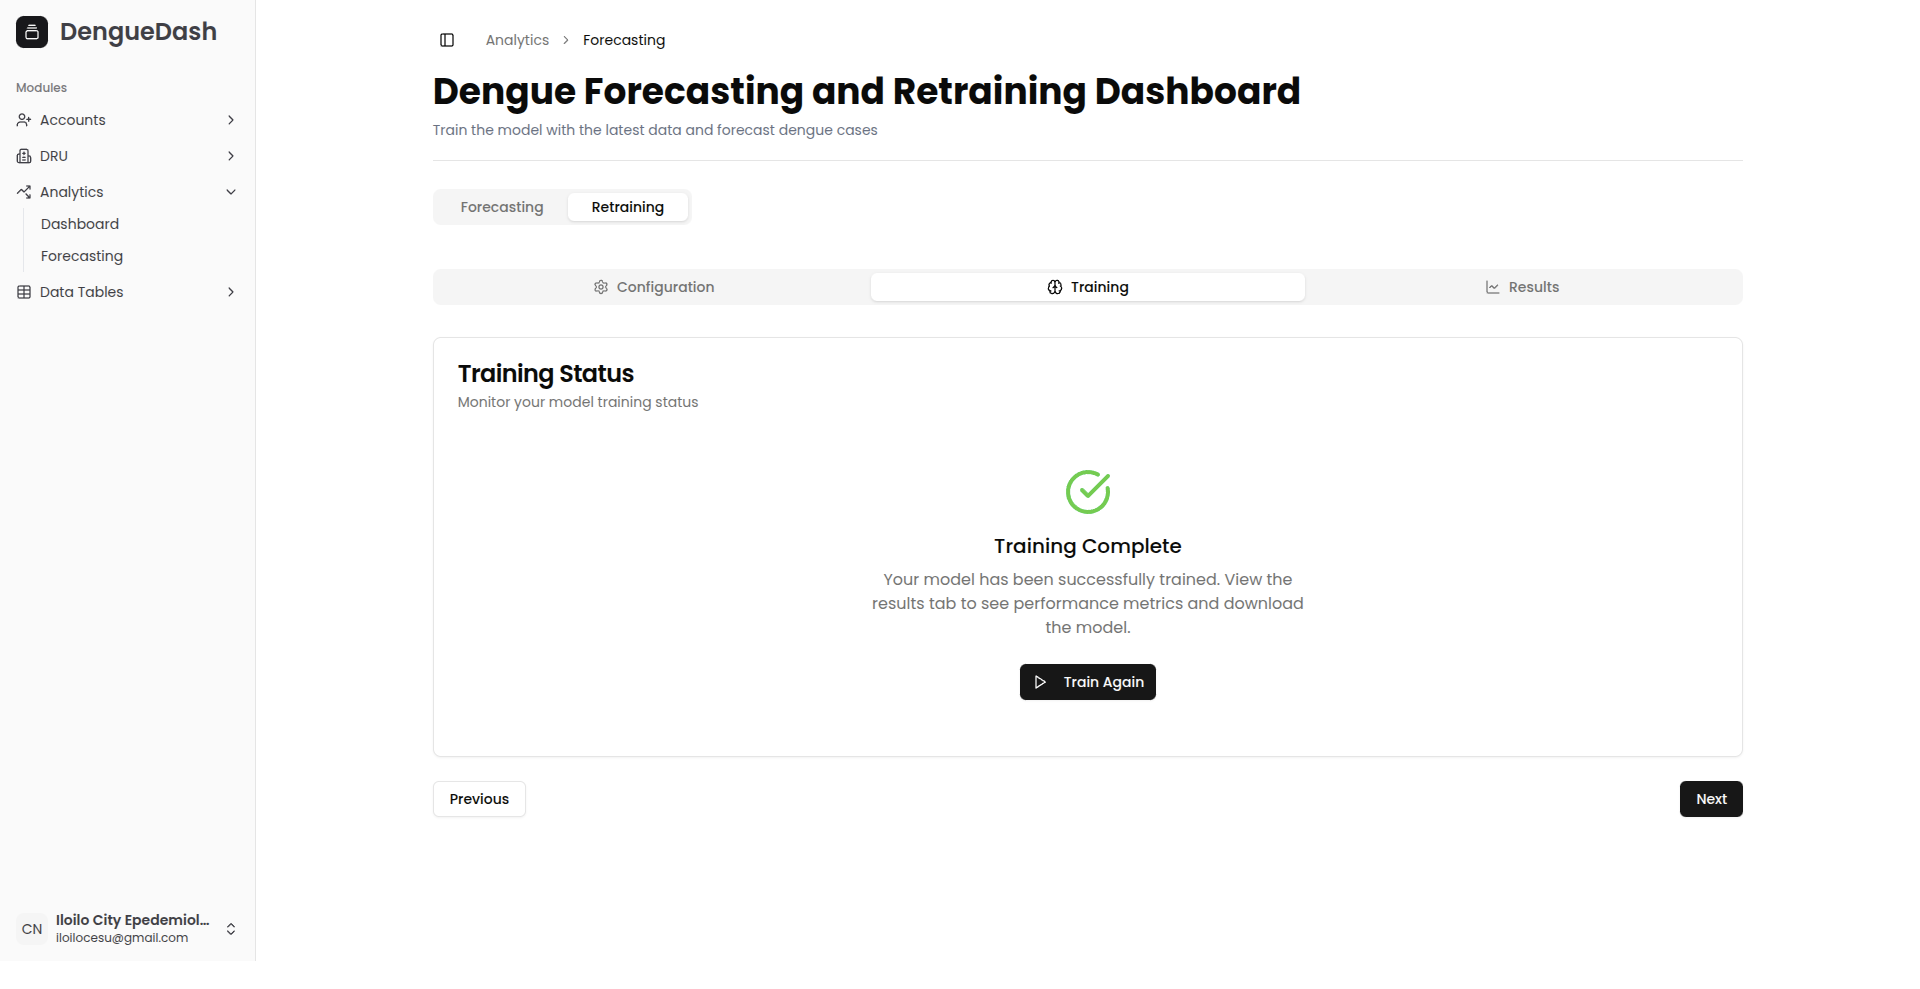
\includegraphics[width=1\textwidth]{retraining_results}
	\caption{Retraining Results}
	\label{fig:retraining_results}
\end{figure}

\subsubsection{Managing Accounts}

Proper management of accounts is important to protect the integrity and confidentiality of data. Thus, it is crucial for administrators to track their users and control the flow of information. As discussed in the user registration of encoders, admin users from a specific DRU or surveillance unit have the power to grant them access to the web application. Figure \ref{fig:pending_accounts} illustrates the interface for this scenario, as the admins can approve or reject their applications. Once approved, these users can access the features given to encoders and may be promoted to have administrative access, as shown in Figure \ref{fig:account_details}. Both Figure \ref{fig:pending_accounts} and \ref{fig:account_details} also show the expanded details of the user, which include personal information, proof of identification, and brief activity details within the system. When deleting an account, the user's email will be blacklisted and illegible to use when creating another account, and all the cases reported by this user will be soft-deleted. However, the blacklist status can be reverted by clicking the "Unban" button, which would make the user of the email able to register to the web application again as shown in Figure \ref{fig:blacklisted_accounts}. 

\begin{figure}[H]
	\centering
	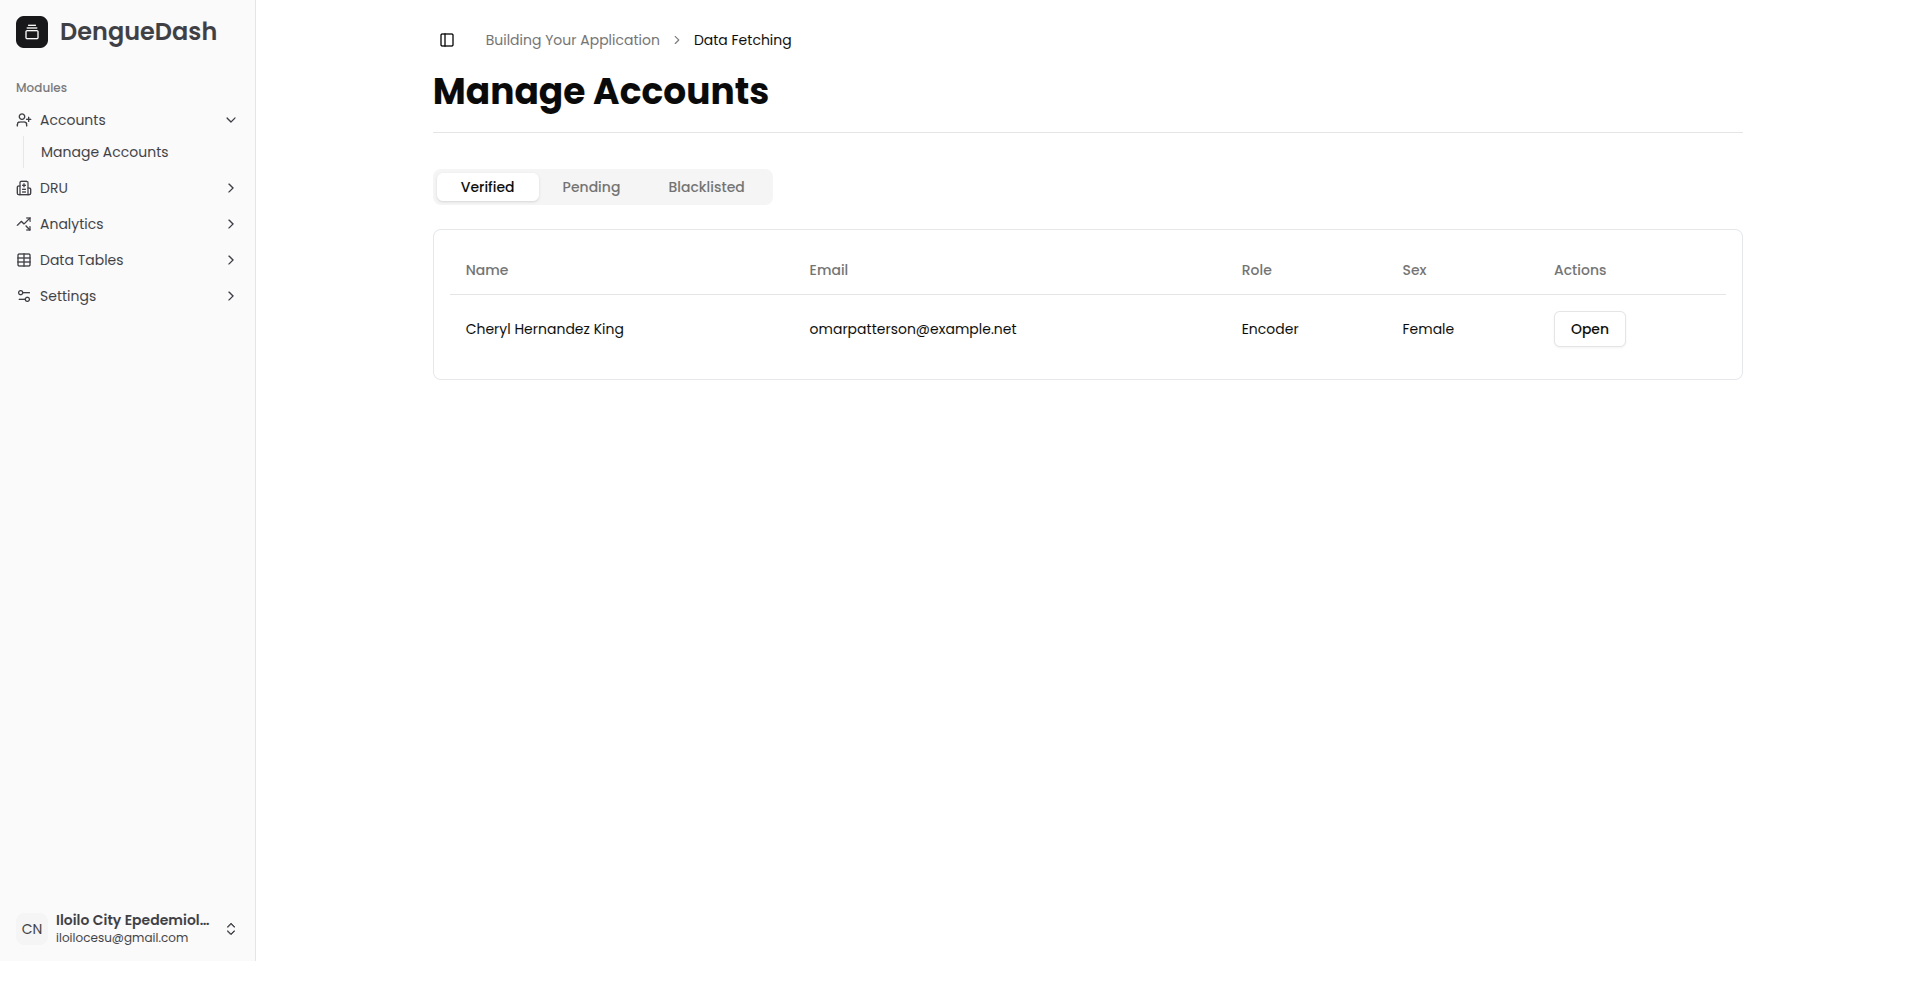
\includegraphics[width=0.8\textwidth]{verified_accounts}
	\caption{List of Verified Accounts}
	\label{fig:verified_accounts}
\end{figure}
\begin{figure}[H]
	\centering
	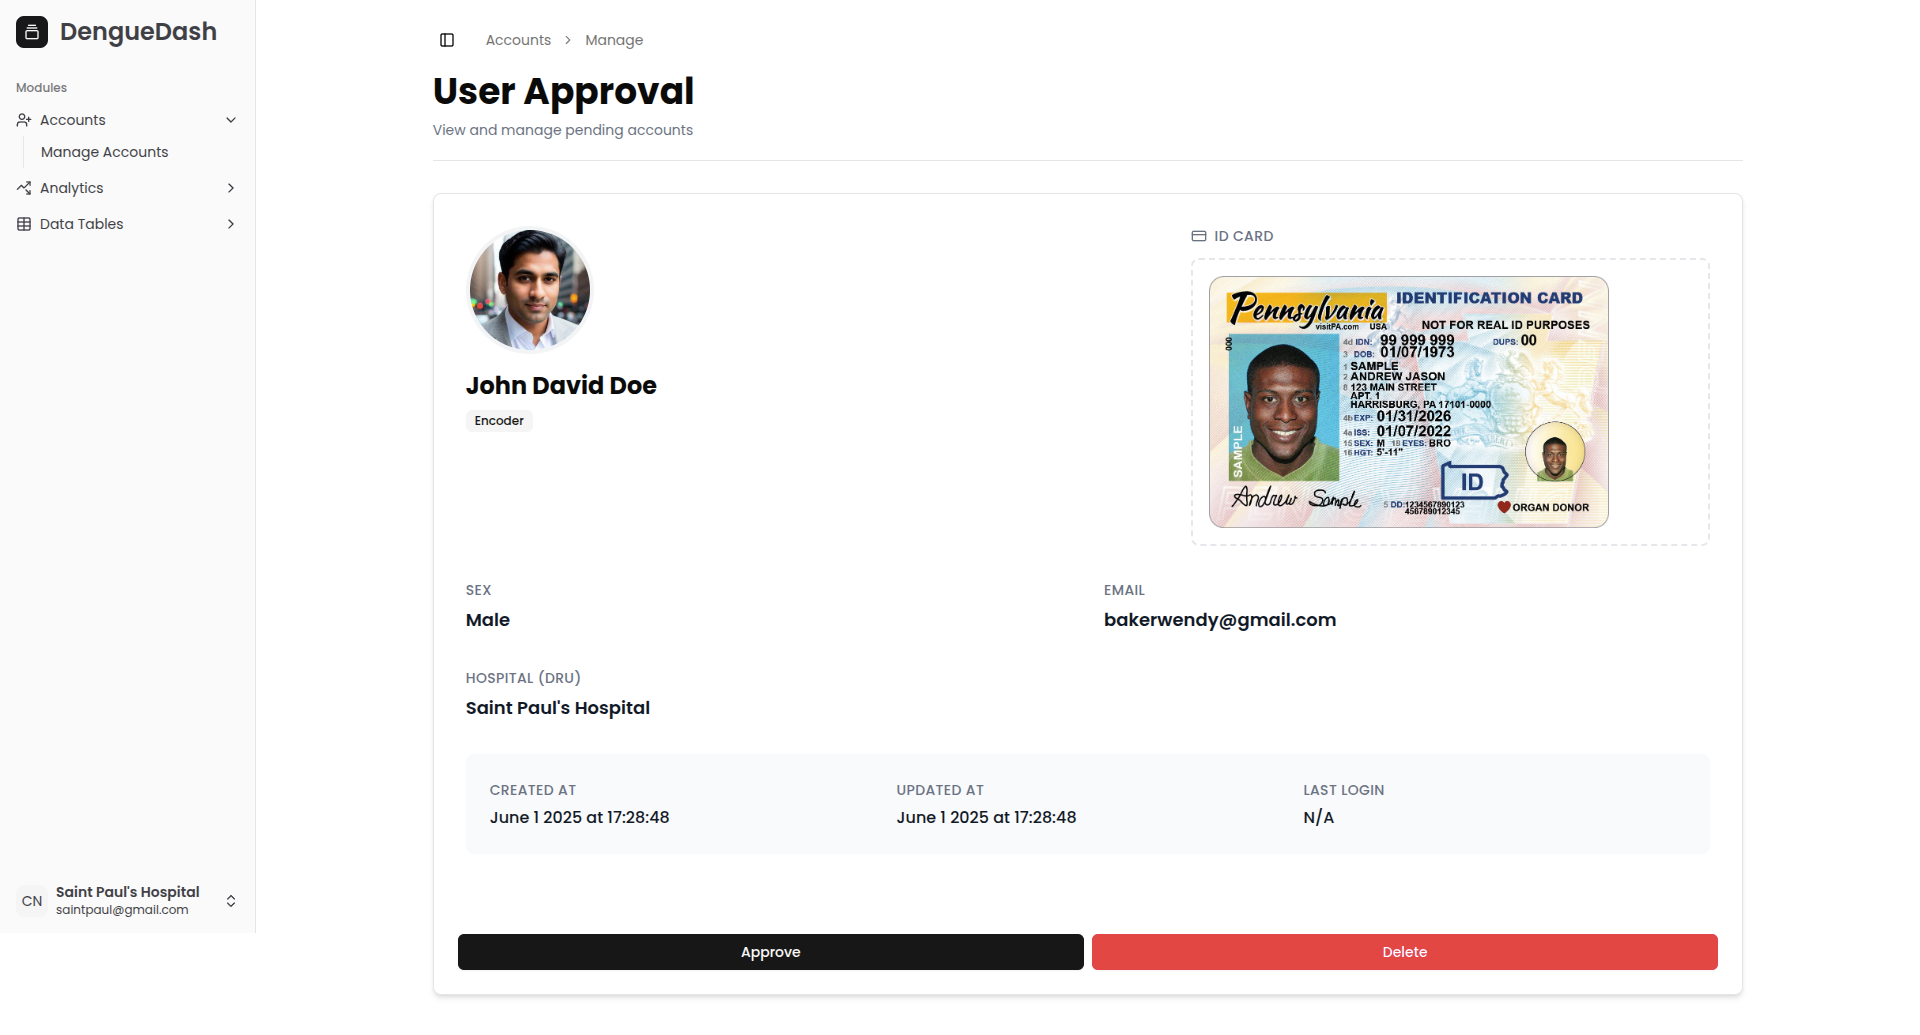
\includegraphics[width=1\textwidth]{pending_accounts}
	\caption{Encoder Approval Page}
	\label{fig:pending_accounts}
\end{figure}
\begin{figure}[H]
	\centering
	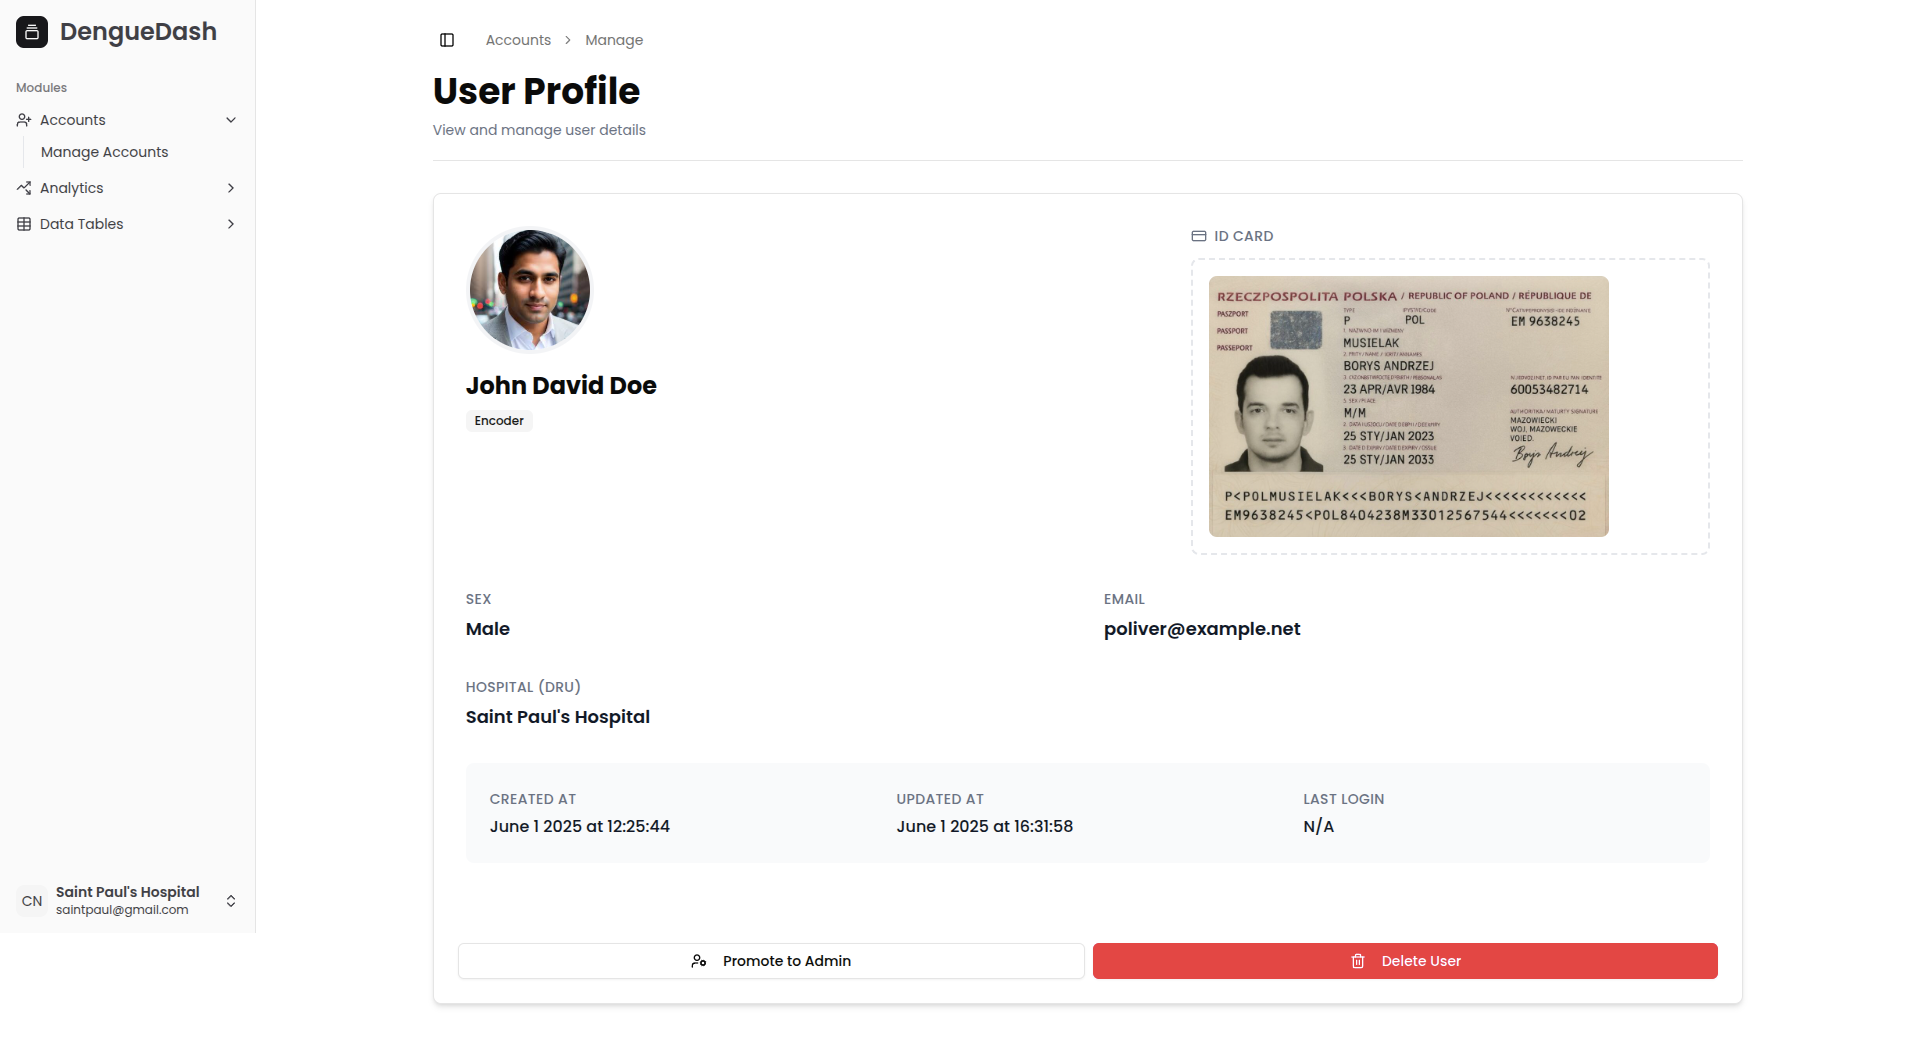
\includegraphics[width=1\textwidth]{account_details}
	\caption{Account Management}
	\label{fig:account_details}
\end{figure}
\begin{figure}[H]
	\centering
	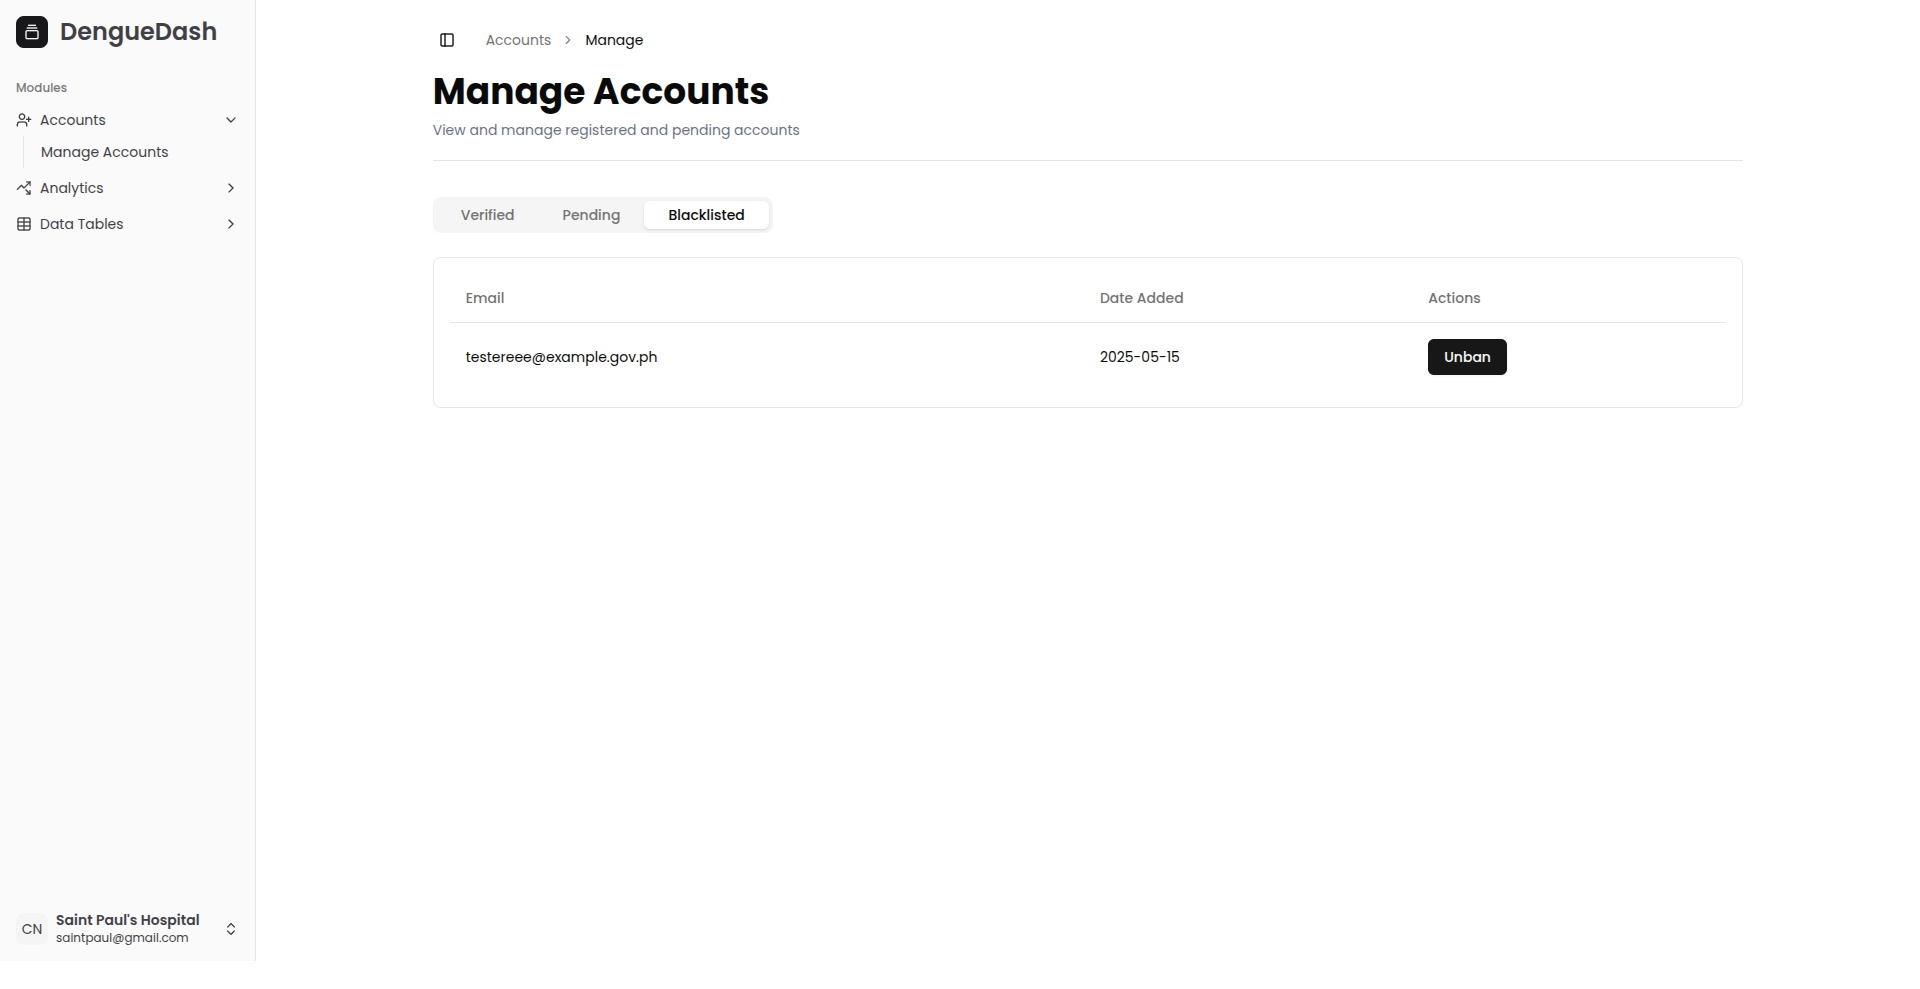
\includegraphics[width=1\textwidth]{blacklisted_accounts}
	\caption{List of Blacklisted Accounts}
	\label{fig:blacklisted_accounts}
\end{figure}

\subsubsection{Managing DRUs}

Unlike the registration of encoder accounts, the creation of Disease Reporting Units can only be done within the web application, and the user performing the creation must be an administrator of a surveillance unit. Figure \ref{fig:register_dru} presents the fields the admin user must fill out, and once completed, the new entry will show as being managed by that unit, as shown in Figure \ref{fig:browse_drus}. Figure \ref{fig:dru_details}, on the other hand, shows the details provided in the registration form as well as its creation details. There is also an option to delete the DRU, and when invoked, all the accounts being managed by it, and the cases reported under those accounts will be soft-deleted.

\begin{figure}[H]
	\centering
	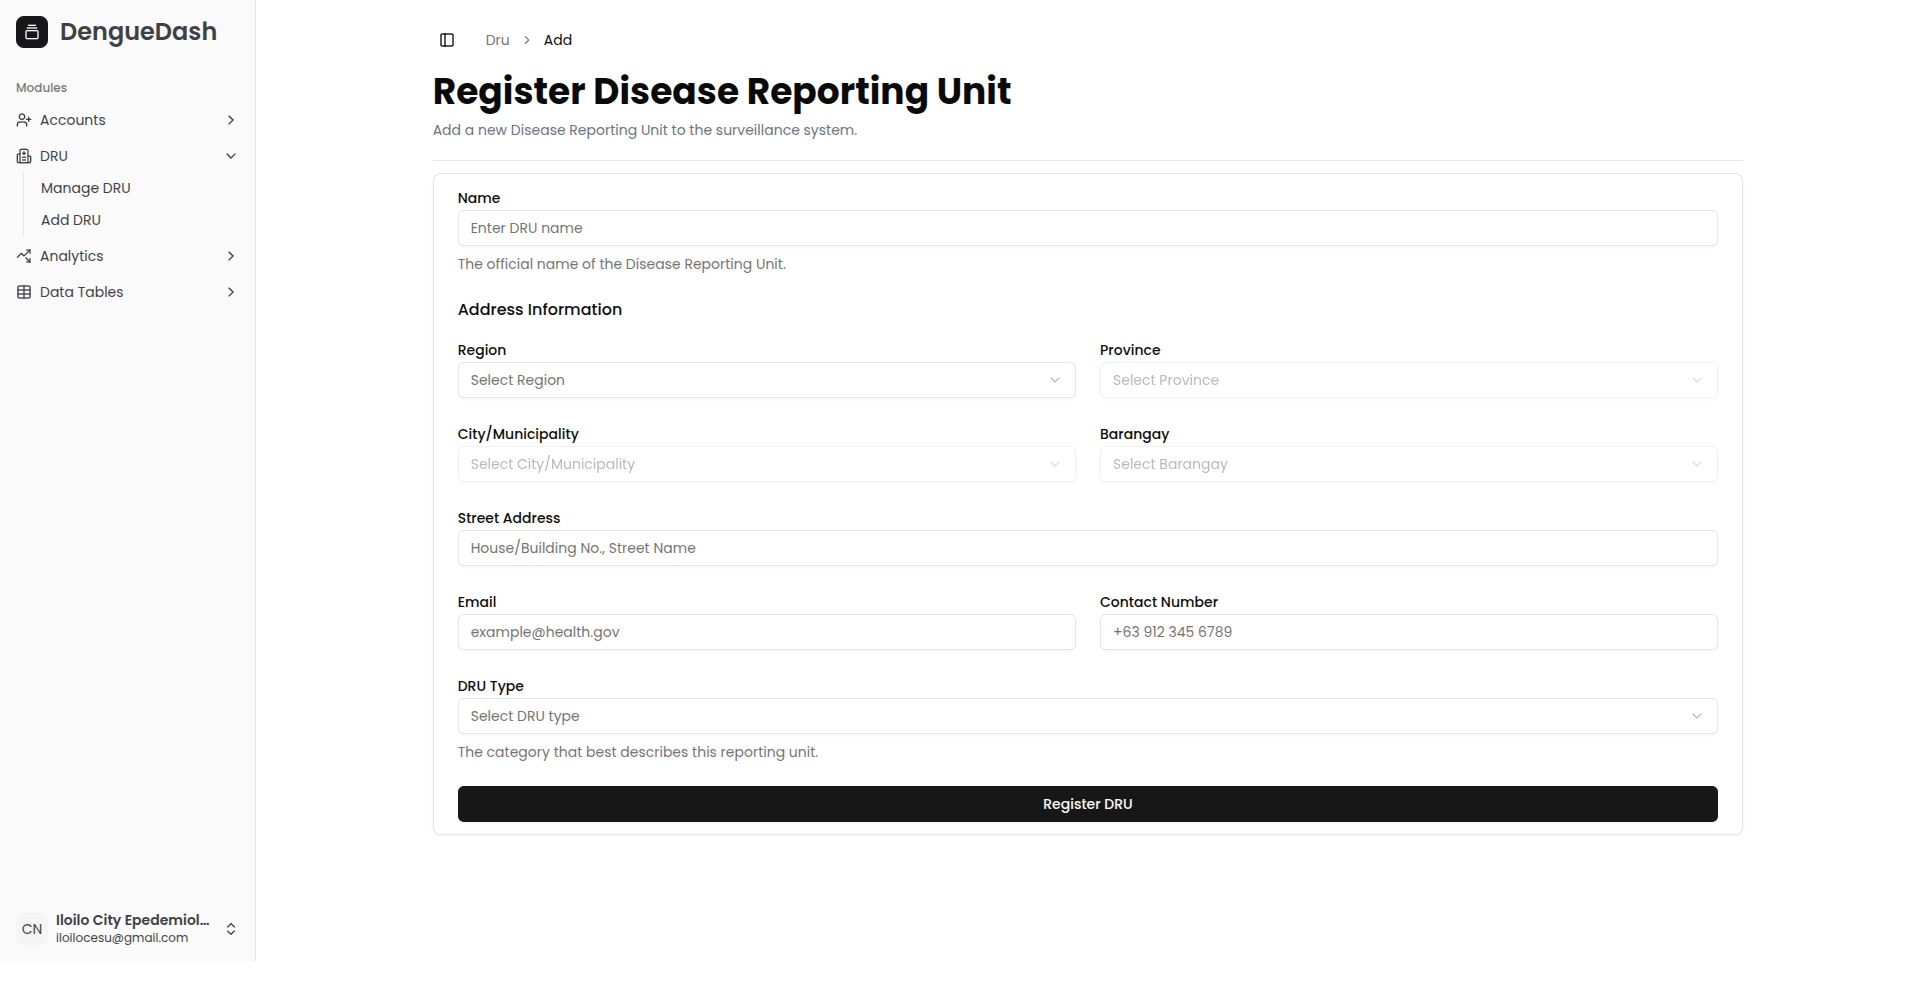
\includegraphics[width=1\textwidth]{register_dru}
	\caption{Disease Reporting Unit Registration}
	\label{fig:register_dru}
\end{figure}
\begin{figure}[H]
	\centering
	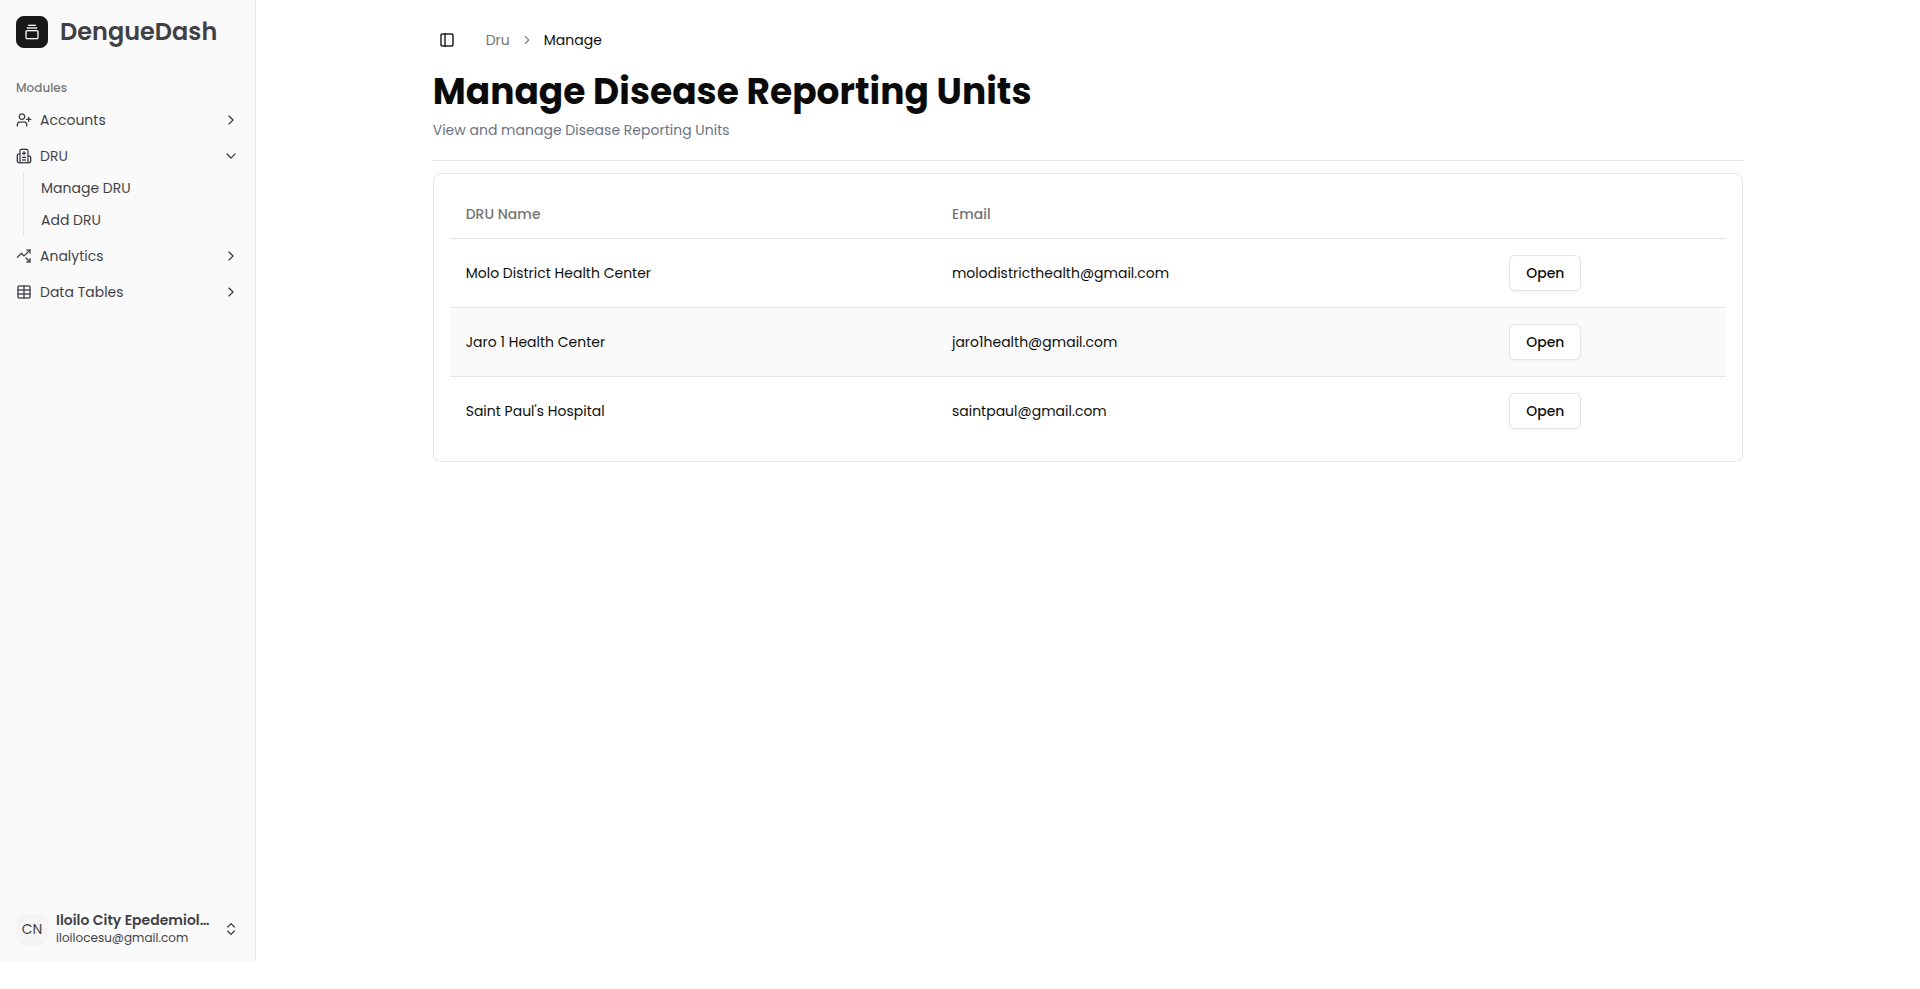
\includegraphics[width=1\textwidth]{browse_drus}
	\caption{List of Disease Reporting Units}
	\label{fig:browse_drus}
\end{figure}
\begin{figure}[H]
	\centering
	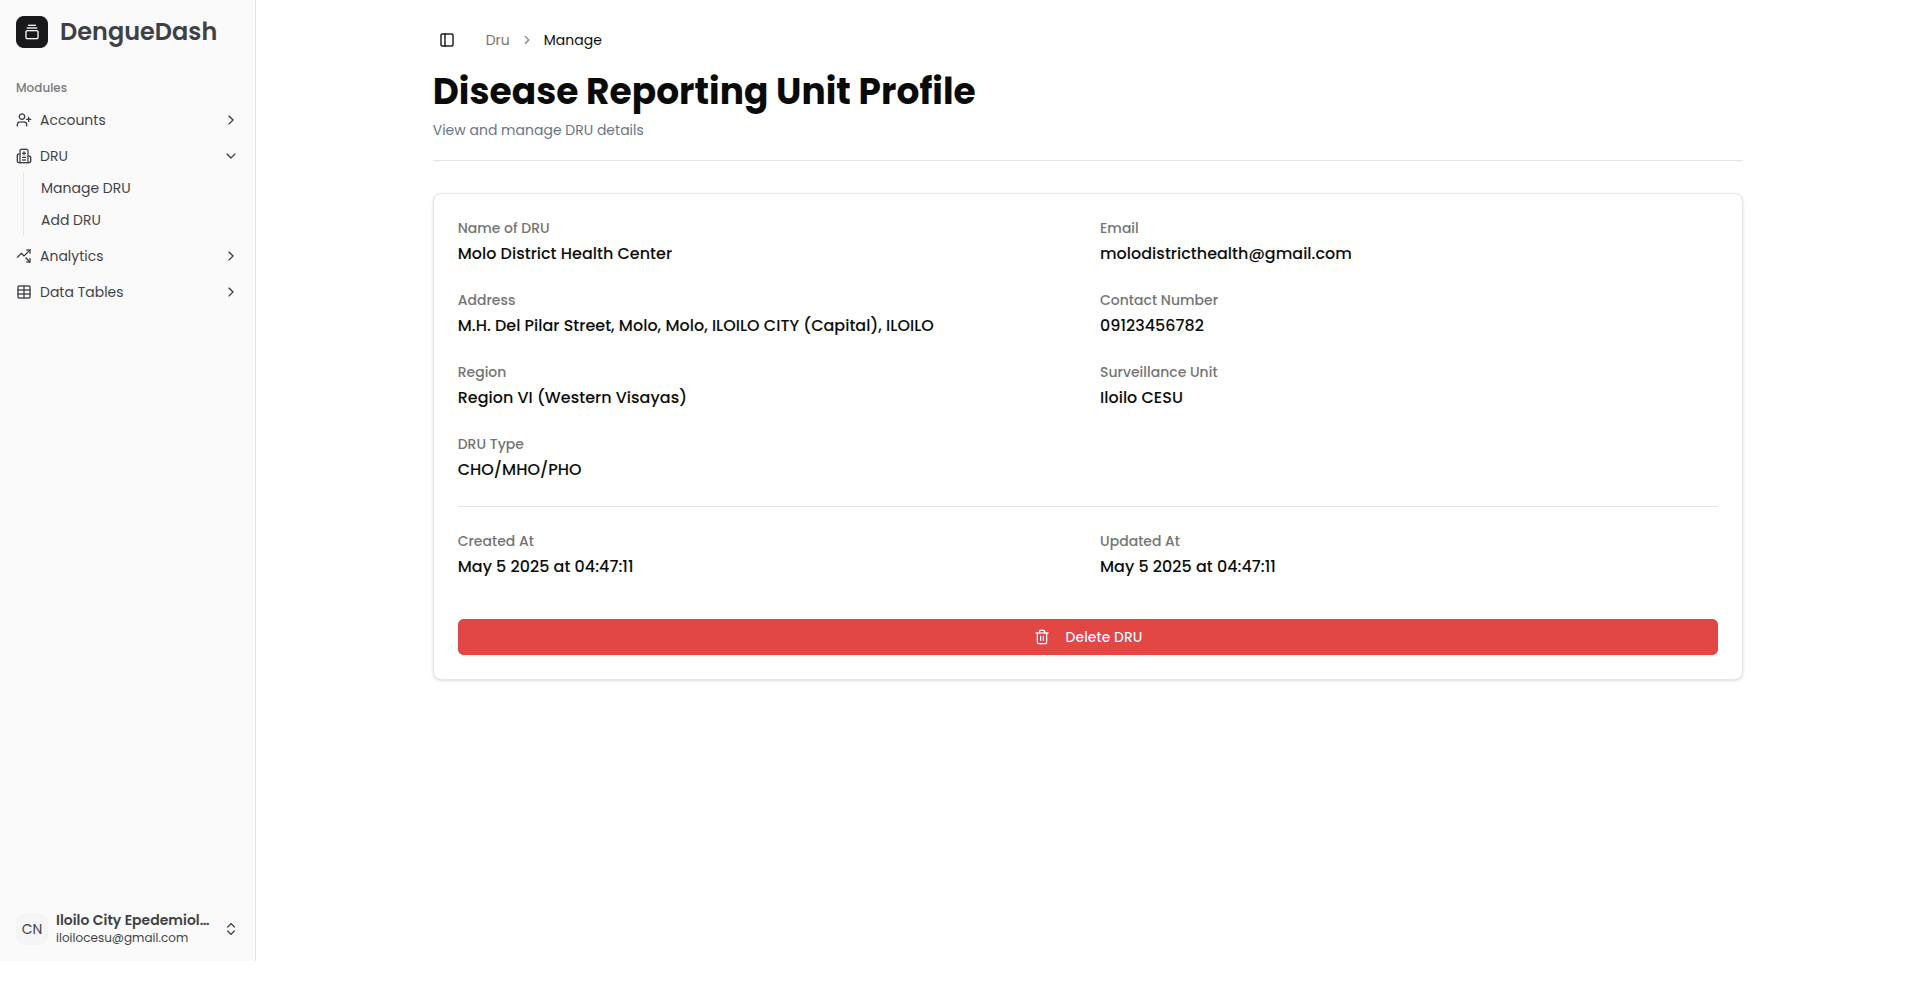
\includegraphics[width=1\textwidth]{dru_details}
	\caption{Disease Reporting Unit details}
	\label{fig:dru_details}
\end{figure}


\section{User Testing}
To evaluate the usability of the system, the System Usability Scale (SUS) was utilized. SUS is a Likert-scale-based questionnaire comprising 10 items that are critical to assessing system usability. A total of five participants completed the survey. Their responses were processed following the step-by-step calculation method adopted from \cite{babich_sus_usability_website}. The resulting usability scores for each participant are shown in Table~\ref{tab:sus_scores}.

\begin{table}[h!]
	\centering
	\begin{tabular}{|c|c|}
		\hline
		\textbf{Participant} & \textbf{Usability Score} \\
		\hline
		1 & 95.0 \\
		2 & 90.0 \\
		3 & 85.0 \\
		4 & 87.5 \\
		5 & 85.0 \\
		\hline
		\textbf{Average} & \textbf{88.5} \\
		\hline
	\end{tabular}
	\caption{Computed System Usability Scores per Participant}
	\label{tab:sus_scores}
\end{table}

The average System Usability Scale (SUS) score across systems is typically 68~\cite{babich_sus_usability_website}. In this testing, the system achieved an average SUS score of 88.5, indicating a highly positive user experience. This score suggests that participants found the system not only enjoyable to use but also intuitive enough to recommend to others. Furthermore, it demonstrates that the system is suitable for real-world applications without presenting significant complexity for first-time users.




